%\documentclass[PhD]{iitmdiss}
%\documentclass[MS]{iitmdiss}
\documentclass[MTech]{iitmdiss}
%\documentclass[BTech]{iitmdiss}
\usepackage{times}
 \usepackage{t1enc}

\usepackage{graphicx}
\usepackage{epstopdf}
%\usepackage[hypertex]{hyperref} % hyperlinks for references.
\usepackage[driverfallback=dvipdfm]{hyperref}
\usepackage{amsmath} % easier math formulae, align, subequations \ldots
\usepackage{algorithm}
\usepackage[noend]{algpseudocode}

\makeatletter
\def\BState{\State\hskip-\ALG@thistlm}
\makeatother

\def\thesistitle{Analysis of Parallel Incremental/Decremental Graph Colouring on GPU}
\def\thesisauthor{Mohammed Shamil}

\begin{document}


%%%%%%%%%%%%%%%%%%%%%%%%%%%%%%%%%%%%%%%%%%%%%%%%%%%%%%%%%%%%%%%%%%%%%%
% Title page

\title{\thesistitle}

\author{\thesisauthor}

\date{MAY 2016}
\department{COMPUTER SCIENCE AND ENGINEERING}

%\nocite{*}
\maketitle

%%%%%%%%%%%%%%%%%%%%%%%%%%%%%%%%%%%%%%%%%%%%%%%%%%%%%%%%%%%%%%%%%%%%%%
% Certificate
\certificate

\vspace*{0.5in}

\noindent This is to certify that the thesis titled {\bf {\thesistitle}}, submitted by {\bf {\thesisauthor}}, 
  to the Indian Institute of Technology, Madras, for
the award of the degree of {\bf Master of Technology}, is a bona fide
record of the research work done by him under our supervision.  The
contents of this thesis, in full or in parts, have not been submitted
to any other Institute or University for the award of any degree or
diploma.

\vspace*{1.5in}
\hspace*{-0.25in}
\begin{singlespace}
\noindent {\bf Dr. Rupesh Nasre} \\
\noindent Research Guide \\ 
\noindent Assistant Professor \\
\noindent Dept. of Computer Science and Engineering\\
\noindent IIT Madras, 600 036 \\
\end{singlespace}
\vspace*{0.25in}
\noindent Place: Chennai\\ 
Date: 11 May, 2016


%%%%%%%%%%%%%%%%%%%%%%%%%%%%%%%%%%%%%%%%%%%%%%%%%%%%%%%%%%%%%%%%%%%%%%
% Acknowledgements
\acknowledgements

Thanks to all those who made \verb+Shamil+ what he is today.
\\
Thank God.
%%%%%%%%%%%%%%%%%%%%%%%%%%%%%%%%%%%%%%%%%%%%%%%%%%%%%%%%%%%%%%%%%%%%%%
% Abstract

\abstract

\noindent KEYWORDS: \hspace*{0.5em} \parbox[t]{4.4in}{Colour Quality; Compressed Sparse Row Representation; Decremental Graph Colouring; GPGPU; Graph Colouring; Incremental Graph Colouring; NP-hard; NVIDIA CUDA; Parallel Computing; Parallel Graph Algorithms; Vertex Colouring.}

\vspace*{24pt}

\noindent To be filled. 

\pagebreak

%%%%%%%%%%%%%%%%%%%%%%%%%%%%%%%%%%%%%%%%%%%%%%%%%%%%%%%%%%%%%%%%%
% Table of contents etc.

\begin{singlespace}
\tableofcontents
\thispagestyle{empty}

\listoftables
\addcontentsline{toc}{chapter}{LIST OF TABLES}
\listoffigures
\addcontentsline{toc}{chapter}{LIST OF FIGURES}
\end{singlespace}


%%%%%%%%%%%%%%%%%%%%%%%%%%%%%%%%%%%%%%%%%%%%%%%%%%%%%%%%%%%%%%%%%%%%%%
% Abbreviations
\abbreviations

\noindent 
\begin{tabbing}
xxxxxxxxxxx \= xxxxxxxxxxxxxxxxxxxxxxxxxxxxxxxxxxxxxxxxxxxxxxxx \kill
\textbf{IITM}   \> Indian Institute of Technology, Madras \\
\textbf{RTFM} \> Read the Fine Manual \\
\textbf{GPU} \> Graphics Processing Unit \\
\textbf{GPGPU} \> General-Purpose computing on Graphics Processing Units  \\
\textbf{CSR} \> Compressed Sparse Row \\

\end{tabbing}

\pagebreak

%%%%%%%%%%%%%%%%%%%%%%%%%%%%%%%%%%%%%%%%%%%%%%%%%%%%%%%%%%%%%%%%%%%%%%
% Notation

%\chapter*{\centerline{NOTATION}}
%\addcontentsline{toc}{chapter}{NOTATION}
%
%\begin{singlespace}
%\begin{tabbing}
%xxxxxxxxxxx \= xxxxxxxxxxxxxxxxxxxxxxxxxxxxxxxxxxxxxxxxxxxxxxxx \kill
%\textbf{$r$}  \> Radius, $m$ \\
%\textbf{$\alpha$}  \> Angle of thesis in degrees \\
%\textbf{$\beta$}   \> Flight path in degrees \\
%\end{tabbing}
%\end{singlespace}
%
%\pagebreak
\clearpage

% The main text will follow from this point so set the page numbering
% to arabic from here on.


\pagenumbering{arabic}
%%%%%%%%%%%%%%%%%%%%%%%%%%%%%%%%%%%%%%%%%%%%%%%%%%
% Introduction.


\chapter{INTRODUCTION}
\label{chap:intro}
Graphs are a well studied and widely used data structure in the field of algorithms, programming and computing. There are a lot of interesting applications of graphs and various algorithms are built on top of the graph data structure. One of the most famous and well studied graph problems is that of graph colouring. There are a lot of different versions of graph colouring problem of which the most common ones are that of vertex colouring and edge colouring. The problem is seemingly simple, to allocate a colour to every vertex/edge of a graph so that adjacent vertices/edges don't share the same colour minimizing the number of colours used.  
Graph colouring is a very important and yet very challenging graph problem with ongoing active research. Graph colouring finds application in a varied range of problems including various scheduling problems like job scheduling on distributed computing systems, register allocation in compilers, pattern matching problems and solving Sudoku boards.

Though the problem is seemingly simple, it is computationally hard. The graph colouring problem we are exploring in this work, that of vertex colouring, is an NP-hard problem. The sequential approaches like greedy colouring are simply not fast enough whereas advanced approximate/randomized solutions either produce colourings of bad colour quality or aren't fast enough. Thus came the parallel approaches to Graph Colouring. Most of the parallel versions of Graph Colouring algorithms were designed with either multi-core CPUs or heavy duty supercomputers in mind. With the advent of General-Purpose computing on GPUs (GPGPU), we have access to cheap heavy multi-threaded parallel computing power. Our work is based on parallel computing on NVIDIA GPUs using CUDA programming language.

We explore different parallel graph colouring algorithms on NVIDIA GPUs in this work and try to adapt them to support addition of edges, called incremental graph colouring, and deletion of edges, called decremental graph colouring. In the first section, we explore different parallel graph algorithms and adapt a couple of them, one based on \textit{speculation} and \textit{conflict resolution} and the other on \textit{Vertex Independent Sets}, to work on NVIDIA GPUs. In the following sections, we adapt the GPU parallel colouring algorithm to support additions and deletions of edges. In the incremental part, we explore different methods to maximize parallelization while colouring newly added edges and use propagation to improve overall colour quality. In the decremental part, we explore different options to either process the vertices, on which the deleted edges were incident, on the go or to process them together and use propagation to propagate the information across the graph improving the colour quality. 
\chapter{Background}
\section{Graphs and Graph Algorithms}
Graphs are really important mathematical concepts and in the area of computing, their various forms are widely used as data structures to aid various algorithms. Graphs are commonly used to denote relations between different entities and hence is a very important and integral part of many algorithms. On a practical level, we deal with graphs in the order of billions of nodes and edges on a daily basis. Especially with the advent of social networks and big data, a lot of active research is ongoing in the analysis and understanding of large graphs.

Many problems in the area of Computer Science, Biology etc. are solved with the help of algorithms which are based on graphs. Shortest path problem, Travelling Salesman Problem (TSP), network flow problems, vertex cover problem, graph colouring etc. are important graph-based problems with many practical applications in the real world. Our work is on Graph Colouring which is one of the most famous and well studied graph problems.
\section{Vertex Colouring}
Graph Colouring problem entails \textit{colouring/labeling} of the vertices/edges of a graph based on some set of conditions which are to be satisfied \citep{jensen2011graph}. In other words, it's a problem in which you allocate a colour/number to every vertex/edge of a graph such that a set of constraints are satisfied. There are different versions of Graph Colouring and the one which is of interest to us is that of Vertex Colouring.
\subsection{Classical Vertex Colouring Problem}
Vertex Colouring is the most basic version of Graph Colouring and other Graph Colouring problems can be presented as a Vertex Colouring problem. In its classical form, Vertex Colouring is:
\begin{verse}
\textit{\textbf{Vertex Colouring:} Colouring all the vertices of a graph such that adjacent vertices have different colours. That is, there shouldn't be an edge where the incident vertices share the same colour.}
\end{verse}
There are other forms of vertex colouring where additional conditions than the one given above need to be considered while colouring. In our work, we are concerned only with the classical form of vertex colouring which hereinafter interchangeably referred to simply as Graph Colouring. An example of Vertex Colouring is given in Figure \ref{fig:colouring}. Vertex \textit{v4} is coloured initially with blue (\textit{b)} colour. Then, its neighbours, vertices \textit{v3, v5, v6 and v2} are coloured with red (\textit{r)} colour. As \textit{v1} has \textit{v2 and v3} also as its edges, it can't take colour red (\textit{r}). So, it's coloured with a new colour, green (\textit{g}).

\begin{figure}[h]
    \centering
    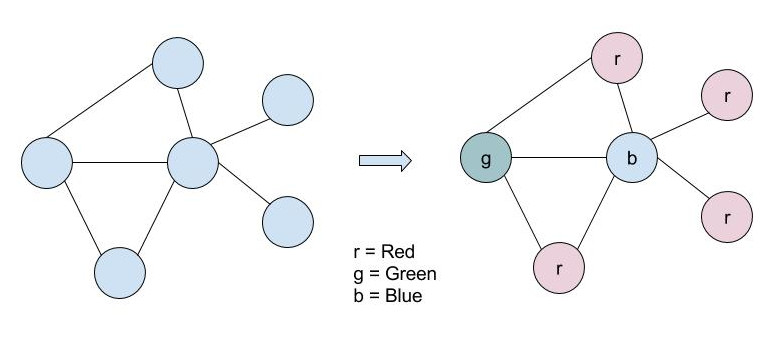
\includegraphics[width=\textwidth,scale=1,keepaspectratio=true]{graphcolouring.jpg}
    \caption{
        Vertex Colouring of a given graph using 3 colours.
    }
    \label{fig:colouring}
\end{figure}

\subsection{Chromatic Number $ \chi(G) $}
A graph \textit{G} is said to \textit{k-}colourable, if \textit{G} can be coloured using \textit{k} colours. For example, from the \textit{Four Colour Theorem} \citep{appel1977, thomas98, wilson14}, we have that all planar graphs are 4-colourable. Also, all bipartite graphs are 2-colourable.
 
\begin{verse}
The \textit{Chromatic Number} of a graph G, denoted by $ \chi(G) $, is the minimum number of colours required to colour a graph. That is, $ \chi(G) $, is the minimum value of all \textit{k} for which the graph \textit{G} is \textit{k-}colourable. 
\end{verse}

For example, $\chi(G)$ of the graph given in Figure \ref{fig:colouring} is 3. Also, it follows that if a graph is \textit{k-}colourable, we have:
\begin{center}
$ \chi(G) \leq k $
\end{center}
\subsection{Colour Quality}
Colour Quality is a term used to denote how good the colouring done by a particular algorithm is. Colour Quality is said to be better for an algorithm if the number of colours used by the algorithm to colour a graph \textit{G} is closer to its Chromatic Number, $\chi(G)$.

Mathematically, Colour Quality of a colouring is said to be better as the fraction,
\begin{center}
$\frac{No. \: of \: colours \: used \: by \: the \: algorithm}{\chi(G)} $
\end{center}
is closer to 1.
\subsection{Complexity}
Graph Colouring is a computationally complex problem. To decide if a Graph can be coloured using \textit{k} colours, is an NP-complete problem. Whereas, finding the Chromatic Number of a graph ($ \chi(G) $) is proved to be an NP-hard problem.

There exist many algorithms like Greedy Colouring, approximation algorithms and randomized algorithms. There also exist polynomial time algorithms for some specific family of graphs. For example, it can be decided if a graph can be coloured using 2 colours by checking if it is a bipartite graph. This can be done in polynomial time using Breadth First Search (BFS).
\subsection{Applications}
Graph Colouring problem, which started as a map colouring problem (four colour theorem), finds many important real applications including but not limited to:
\begin{itemize}
\item Scheduling problems like job scheduling across multiple nodes in a distributed computing environment \citep{leighton1979graph}
\item Register allocation problem during compilation \citep{Briggs:2004:CHR:989393.989424}
\item Solving Sudoku \citep{herzberg2007sudoku}
\item Applications on biological networks like Protein-Protein Interaction (PPI) Networks \citep{khor2009application}
\item Scheduling cell-transmissions in an ATM switch \citep{lakshman1994graph}
\end{itemize}
\section{Parallelization}
\subsection{Frequency Scaling}
\begin{figure}[h]
    \centering
    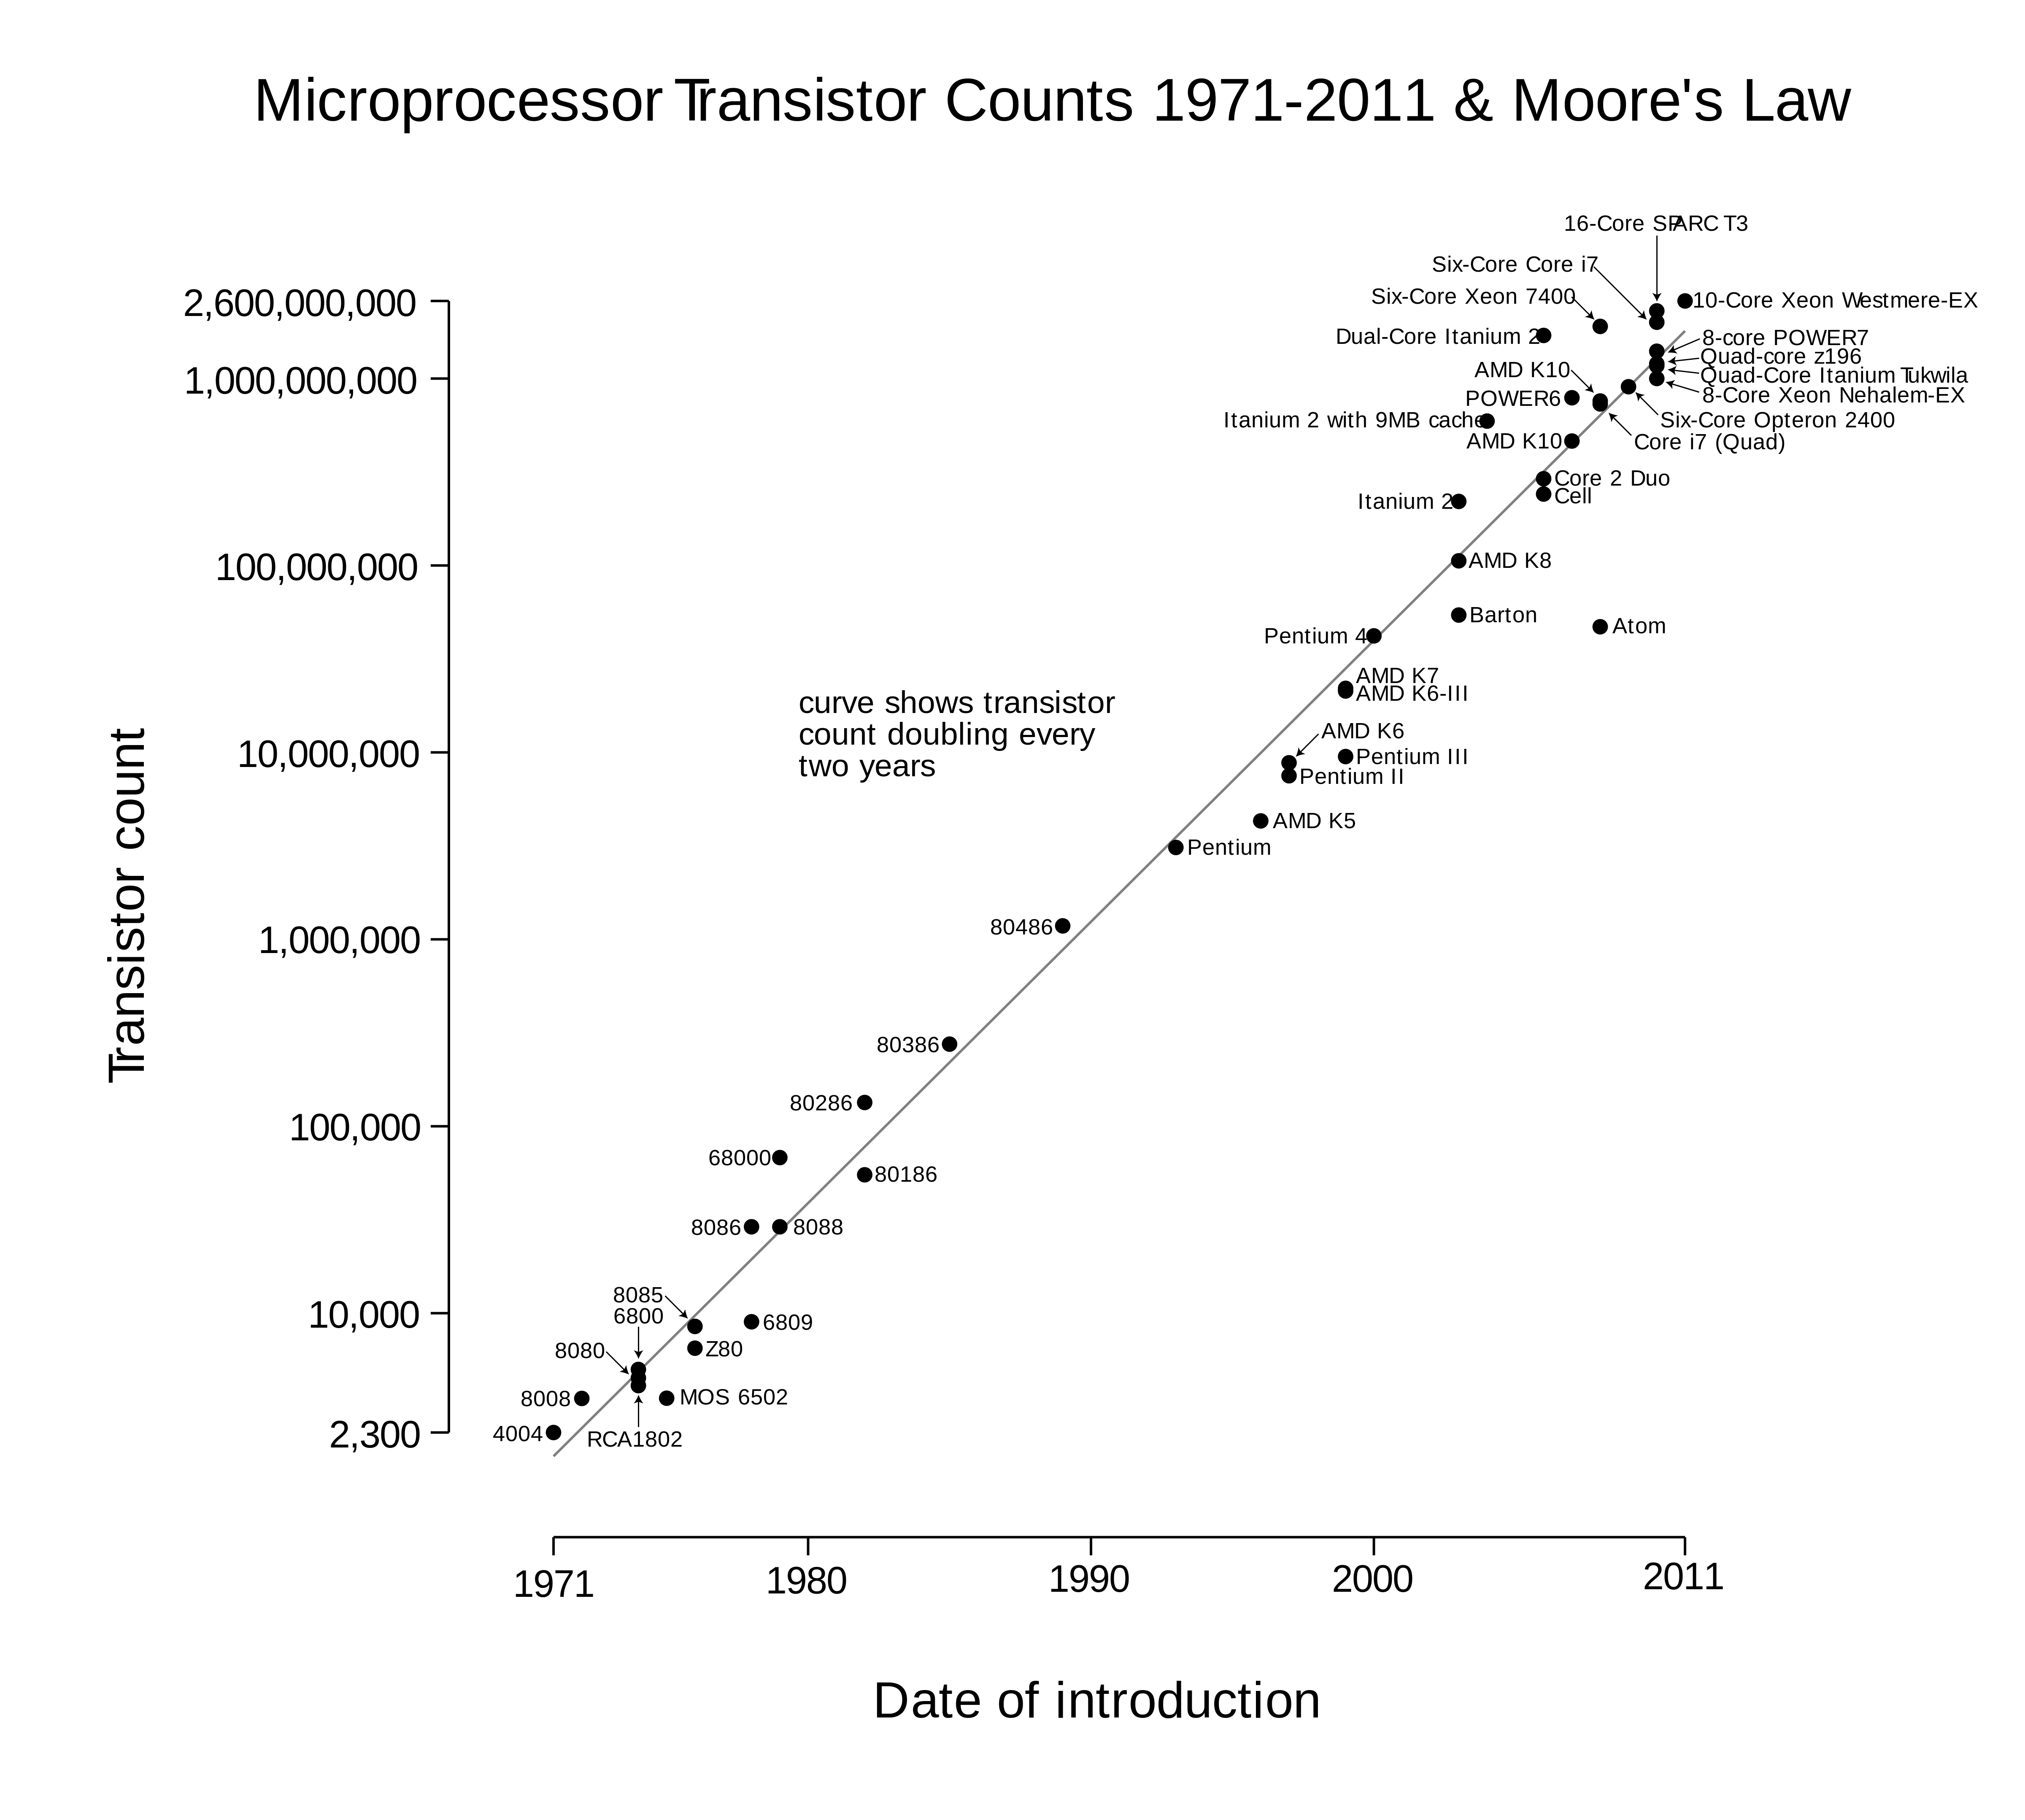
\includegraphics[width=\textwidth,scale=0.6,keepaspectratio=true]{mooreslaw.jpg}
    \caption{
        Graph showing Moore's Law in action, from \cite{WikipediaEN:ML}. Each data point is a processor.
    }
    \label{fig:moore's law}
\end{figure}
Moore's law, which observes that the number of transistors present in an integrated circuit approximately doubles every two years, still stands valid. Processors, and hence computers, have grown faster and faster over years. More and more transistors meant the processors could run faster, at a faster frequency. Processors with better and better clock speeds were introduced every year since the 1980s until around 2004 when instead of single core processors running at faster clocks or higher clock speeds, multi-core processors started rolling out.
\subsection{Why Parallelization?}
\begin{figure}[h]
    \centering
    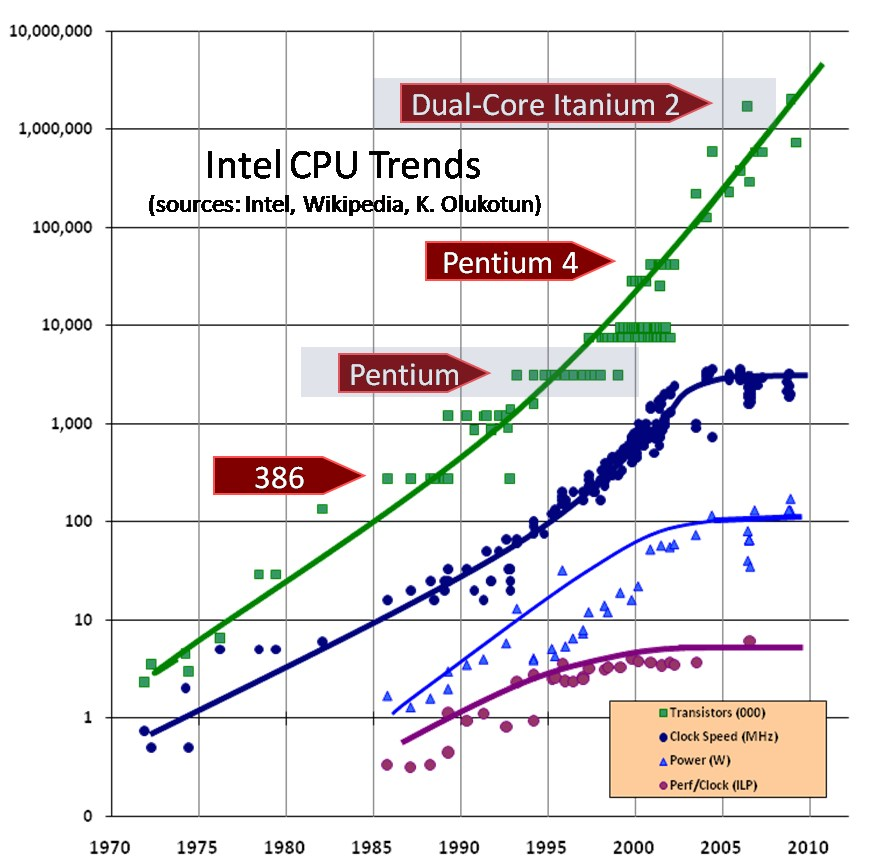
\includegraphics[width=\textwidth,scale=0.6,keepaspectratio=true]{CPU-Scaling.jpg}
    \caption{
        \textit{Intel}'s transition from single core processors to multi-core processors around 2004-2005, from \cite{Herb:Intel}.
    }
    \label{fig:intel}
\end{figure}
Around 2004, Intel and other processor manufacturing companies came to realize that frequency scaling was not practical any more. The increase in frequency meant an increase in power consumption which in turn meant an increase in heat generation. Thus it was no longer practical to increase the clock speeds of processors. Rather, they started making processors with the same clock speeds, but with multiple cores. Since then the computer architecture industry held fast to the paradigm of multi-core processors. This, in the case of \textit{Intel}, is indicated in the figure \ref{fig:intel}.

Parallelization enables us to run programs faster by splitting the work across different cores of a processor which are ideally run in parallel. In an ideal setup, with \textit{n} cores, we should see a speed up of \textit{n}, which means the running time will become $1/n^{th}$ compared to the running time when run on a single core processor. Though we rarely really reach this ideal speedup, as stated by Amdahl's law \citep{Amdahl:1967:VSP:1465482.1465560} etc., we still achieve significant speed ups.
\subsection{Parallelization of Graph Colouring}
Since the computer architecture industry made a shift to the multi-core paradigm, there had to be a shift in programming paradigm to support the newly available parallelism. Almost all the algorithms, programs etc. were designed and developed to run sequentially on a single core processor. Things have changed recently as more and more algorithms and programs are redesigned and redeveloped to make use of the newly available parallel hardware.

As discussed earlier, Graph Colouring is a computationally complex problem. It is NP-hard to solve. Also, the approximation algorithms for colouring a graph with $n$ vertices are also NP-hard within $n^{1-\epsilon}$ for all $\epsilon > 0$ \citep{Zuckerman:2006:LDE:1132516.1132612}. The existing solutions are either slow or are fast but produce bad colour quality. Also, practical graphs these days are very large with billions of vertices and edges. So, since the advent of parallel programming paradigms, there have been efforts to parallelize this well-celebrated graph problem though most of them were meant specifically for distributed computing setups \citep{journals/jpdc/BozdagGMBC08, DBLP:conf/hpcc/BozdagCGMBO05} and supercomputers \citep{CAtalyuRek:2012:GCA:2396901.2397093}. In our work, we focus on parallel graph colouring which can be run on parallel hardware available locally. Especially with the advent of GPGPUs, cheap massive parallelism is at a hand's reach.
\section{GPGPU}
In the domain of parallel programs and applications, one big deterrent was that the number of processor cores available for parallelism was small. Most of the multi-core processors have 32 cores at the maximum. Only supercomputers had a very high number of cores and they came at a price. 
\subsection{Why GPUs?}
Graphics Processing Units, GPUs, have been using parallelism since their birth. They have almost always been very accessible to the normal public as they are much cheaper than supercomputers. They also came with thousands of cores. But they were specialized for graphics related operations. Then came the paradigm of GPGPU, General Purpose computing on Graphics Processing Units. With that, it was now possible to run regular operations and not just graphics related operations on the GPU. GPGPU brought with it easy, cheap access to massive parallelism.
\subsection{NVIDIA CUDA}
NVIDIA, one of the biggest players in the GPUs market, introduced its famous parallel computing platform, CUDA, in 2006, thus enabling easy GPU based parallel acceleration. In our work, we use CUDA C to parallelize graph colouring. CUDA lets us harness the power of thousands of cores in the CUDA enabled NVIDIA GPUs.
\subsubsection{Architecture}
\begin{figure}[h]
    \centering
    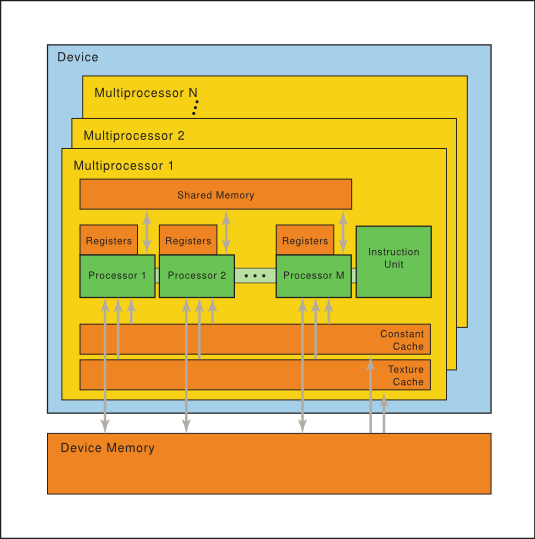
\includegraphics[width=\textwidth,scale=0.4,keepaspectratio=true]{hardware-model.png}
    \caption{
        NVIDIA GPU hardware model, from \cite{nVidia:Hardware}.
    }
    \label{fig:nvidia}
\end{figure}
In an NVIDIA GPU, as shown in the figure \ref{fig:nvidia}, there are multiple streaming multi-processors, SMs, and each of these multi processors have thousands of cores/processors in it. Functions to be executed on the GPU are called Kernels and Kernels, once invoked, spawn the required number of threads as blocks of threads which are then executed across SMs. All threads in a block have access to the shared memory inside the SM in which that block is executed.
\subsection{Challenges}
Though, GPUs let us access thousands of threads easily, it comes with a cost \citep{Lee:2010:DGV:1816038.1816021}. In discrete GPUs like the NVIDIA GPUs used in our work, GPU memory and CPU memory are mutually exclusive. So, we have to first copy all the data which are to be processed by the GPU threads to the GPU before invoking the kernels. As the communication between the CPU and the GPU is enabled through the PCI-Express Bus, which is not super fast with bit rates at around \verb+5 Gbits/sec+, and the fact that while transferring data, we force the CPU to wait for the GPU, there is a cost for transferring data between the CPU and the GPU, the so called \textit{memory latency}. This data transferring cost is one of the biggest overheads in GPU computing \citep{hovland2008latency}. So, as a GPU programmer, one must try to reduce data transfer between the CPU and the GPU. Also, GPUs are not yet ready to do everything that a normal CPU does.  
\section{Incremental/Decremental}
As we discussed already, Graph Colouring is a very important problem on graphs. We have so many practical applications for the same. But most of the practical graphs are dynamic in nature. Vertices and edges are added and deleted often. But the number of these changes is very small compared to the size of the full graph. So, it follows that it is not wise to rerun the graph colouring algorithm on the entire graph every time some vertices/edges are added or deleted. Our work on Incremental/Decremental graph colouring tries to take care of precisely the same.

In our work, we try to re-colour only the relevant parts of the graphs on addition/deletion of edges instead of re-colouring the entire graph. We consider only addition/deletion of edges as deletion of a vertex is considered as the deletion of all edges incident on that vertex. We consider different implications of Incremental/Decremental colouring such as the amount of time we save versus maintaining/improving the colour quality.

\chapter{PARALLEL GRAPH COLOURING}
We have established why we are interested in the paradigm of parallel programming and why we want to parallelize graph colouring.
\section{Graph Colouring Problem}
The problem we are concerned with is that of \textit{1-distance Vertex Colouring} or simply, \textit{Vertex Colouring}.
\begin{verse}
\textit{\textbf{Parallel 1-distance Vertex Colouring:} Colouring all \textit{V} vertices of a graph \textit{G(V,E)} in parallel, such that vertices at a distance of 1 edge, adjacent vertices, don't share the same colour.}
\end{verse}
\section{Related Work}
Graph Colouring is a well studied problem and there have been so many works on the same over years. But most of them were regarding sequentially solving the problem using various paradigms, like that of semi-definite programming, integer programming etc.

Recently there have been some parallel approaches to the same, but most of them like the works by \citet{journals/jpdc/BozdagGMBC08, DBLP:conf/hpcc/BozdagCGMBO05} and \citet{CAtalyuRek:2012:GCA:2396901.2397093} are based on distributed computing setups, supercomputers or other expensive hardware. There have been only a few work done regarding parallel graph colouring on GPUs like \citet{Grosset:2011:EGC:2038037.1941597}, \citet{nvidia:naumov} and \citet{6828158} and none regarding Incremental/Decremental versions as far as the author understands.
\section{Broad Classification of Parallel Graph Colouring Algorithms}
As we are dealing with NVIDIA GPUs, we are concerning ourselves with algorithms pertaining to shared memory architectures only. Most of the parallel colouring algorithms based on shared memory architecture can be broadly classified into two of the following categories:
\subsection{Vertex Independent Sets and Colouring}
Algorithms falling under this category work in two phases:
\begin{enumerate}
\item Vertex Independent Sets: Find VIS
\item Colouring: Colour the VIS found without conflicts
\end{enumerate}

This set of algorithms relies upon finding  Vertex Independent Sets of vertices and colouring them in parallel. Most of the earlier parallel algorithms developed for graph colouring were based on this idea.

\begin{verse}
Vertex Independent Set (VIS): A vertex independent set of a graph G is a set of vertices who don't have any edges amongst each other.   
\end{verse}

Mathematically, $\gamma$ is a valid Vertex Independent Set of a graph $G(V,E)$ if
\begin{center}
$\gamma \subseteq V$

and

$\forall \: v_{i}, v_{j}\in\gamma$, $e\in E$, if $v_{i}$ is incident on $e$, then $\forall \: j \neq i$, $v_{j}$ is not incident on $e$.
\end{center}

The idea is pretty straightforward. These are iterative algorithms where, in each iteration, you find a Vertex Independent Set of the given graph and colour all of the vertices in that VIS with a single colour. The process is continued with different colours until there are no more vertices to be coloured. Both the steps, finding VIS and colouring the vertices in that VIS, can be done in parallel. This category of algorithms roughly works as explained in Algorithm \ref{VISColouring}.

Phase 1 of the Algorithm \ref{VISColouring} is done in Line \ref{1.1} where we find a VIS of the graph. This step can be parallelized as discussed later in Algorithm \ref{Luby} and Algorithm \ref{MinMaxSet}. Phase 2 of the algorithm, colouring the newly found VIS of the graph, is done in Lines \ref{1.6} and \ref{1.7}. In Line \ref{1.8}, we remove the vertices which were coloured in the current iteration from the graph. We then choose a new colour for the next iteration as in Line \ref{1.9} and return to Line \ref{1.4}. The algorithm iterates until there are no more vertices to be processed.

\begin{algorithm}
\caption{Vertex Independent Sets and Colouring}\label{VISColouring}
\begin{algorithmic}[1]
\Procedure{VISParallelGraphColouring(G(V,E))}{}
\State $\textit{Initialization}$\Comment{Initialize all the variables and other data structures}
\State $\textit{currentColour} \gets 1$
\While{$V\not=\phi$} \Comment{Run until all the vertices are coloured} \label{1.4}
\State $\gamma \gets \textit{a VIS of G(V,E)}$ \Comment{VIS can be found in parallel} \label{1.1}
\For{$each \: v \in \gamma$} \Comment{This loop can be run in parallel} \label{1.6}
\State $\textit{colour[v]} \gets currentColour$ \label{1.7}
\EndFor
\State $V \gets V \: \textbackslash \: \gamma$ \label{1.8}
\State $\textit{currentColour} \gets \textit{currentColour}+1$ \label{1.9}
\EndWhile
\EndProcedure
\end{algorithmic}
\end{algorithm}

\subsection{Speculation and Conflict Resolution}
Algorithms falling under this category work in two phases:
\begin{enumerate}
\item Speculation: Colour the graph based on some pre-existing knowledge possibly generating conflicts
\item Conflict Resolution: Resolve the conflicts possibly generated in the first phase
\end{enumerate}
The first category of algorithms relied upon finding Vertex Independent Sets iteratively so that we could colour the vertices in the VIS found in each step without any conflict. This second category of algorithms instead lets us commit some mistakes, or rather conflicts, in our colouring. That is, it saves us from finding a VIS in each step, instead we colour the graph using some pre-existing knowledge like existing colouring of the graph or some structural information regarding the graph.

So, in the first phase, instead of finding a VIS and colouring just the vertices in that VIS without any conflict in an iteration, we speculate the colours of the entire graph with some pre-existing knowledge and possibly commit conflicts. The possible conflicts inflicted in this first phase are rectified in the second phase in which we find the conflicts and resolve them. For practical reasons, the first phase is done in parallel and the second phase is done sequentially or partially in parallel. This category of algorithms roughly works as explained in Algorithm \ref{SpecColouring}.

Phase 1 of the Algorithm \ref{SpecColouring}, \textit{speculation}, is done in Lines \ref{2.4} and \ref{2.5}. We are not explicitly mentioning how this speculation is done as there are many possible ways to speculate the colours. Some of the ways to speculate colours are discussed in Algorithms \ref{spec1}, \ref{spec2} and \ref{randcolour}. Conflicts are then resolved, mostly using some form of Greedy Colouring, in the phase 2 of the algorithm as in Lines \ref{2.7}, \ref{2.8} and \ref{2.9}. Line \ref{2.8} assumes conflicts are already detected. This \textit{Conflicts Detection} part can be parallelized.

\begin{algorithm}
\caption{Speculation and Conflict Resolution}\label{SpecColouring}
\begin{algorithmic}[1]
\Procedure{SpecCRParallelGraphColouring(G(V,E))}{}
\State $\textit{Initialization}$
\BState \emph{speculation}:
\For{$each \: v \in V$}\Comment{Can be done in parallel} \label{2.4}
\State $\textit{colour[v]} \gets speculatedColour$ \label{2.5}
\EndFor
\BState \emph{conflict resolution}:\Comment{Done serially or partially in parallel}
\For{$each \: v \in V$} \label{2.7}
\If{$\textit{colour[v]}$ has a conflict}\Comment{Conflicts can be found in parallel} \label{2.8}
\State $\textit{colour[v]} \gets$ a new colour which resolves the conflict \Comment{Greedy} \label{2.9}
\EndIf 
\EndFor
\EndProcedure
\end{algorithmic}
\end{algorithm}
\section{Algorithms}
In this section, we will discuss some of the existing graph colouring algorithms belonging to both categories, Vertex Independent Set and Colouring and Speculation and Conflict Resolution, as discussed in the previous section. We also concern ourselves with only those parallel algorithms which are scalable. Hence algorithms like Parallel First Fit graph colouring, the parallel version of the First Fit colouring heuristic, are not considered. 
\subsection{Sequential Greedy Graph Colouring}
We start with discussing a sequential graph colouring algorithm, one of the easiest, the Greedy Colouring algorithm. Many other algorithms, including many parallel graph colouring algorithms, are based on greedy colouring.

In Greedy Colouring, you choose each vertex of the graph and assign it the smallest colour number available which is not currently in use by one of its adjacent vertices. This is described in Algorithm \ref{GreedyColouring}. As is evident, the colour quality produced by Greedy Colouring can be arbitrary. In other words, the colour quality produced will depend on the order in which vertices are processed by the algorithm.

Algorithm \ref{GreedyColouring} proceeds by choosing each vertex in some order, Line \ref{3.3}, and colouring them in a greedy fashion. The order in which the vertices are chosen is very important in deciding the colour quality. There are many ways to decide the order in which the vertices are processed and we assume one of the ways is chosen. We then check the vertex's neighbourhood, Line \ref{3.4}, and if a neighbour is already coloured, Line \ref{3.5}, we mark its colour as unavailable as in Line \ref{3.6}. Now, for the vertex, we check which is the smallest colour less than or equal to $\Delta+1$ (Greedy Colouring uses at most $\Delta+1$ colours, where $\Delta$ is the maximum degree among all the vertices of the graph) that is available. This is done in Lines \ref{3.7} and \ref{3.8}. Then finally we colour the vertex with this new colour as in Line \ref{3.9}. The \verb+availableColours[]+ array is reinitialized to all \textit{TRUE} values in Line \ref{3.11} before the algorithm goes back to Line \ref{3.3}.  

Greedy Colouring can produce a colour quality of $\chi(G)$ for atleast one ordering of the vertices. But, on an average, this heuristic performs far from optimal. But the greedy colouring algorithm gives us an upper bound on the number of colours that it uses. The colouring produced uses at most $\Delta+1$ colours, where $\Delta$ is the maximum degree among all the vertices of the graph. As the order in which the vertices are processed is very important, there have been many approaches suggested over the years which on an average produce a better colour quality. One of them is the so called Welsh-Powell Algorithm \citep{Welsh01011967}, in which we process the vertices in the order of their degrees.
\begin{algorithm}
\caption{Sequential Greedy Graph Colouring}\label{GreedyColouring}
\begin{algorithmic}[1]
\Procedure{GreedyColouring(G(V,E))}{}
\State $\textit{Initialization}$
\For{$each \: v \in V$} \label{3.3}
\For{$each \: u \in V$ adjacent to $v$} \label{3.4}
\If{$\textit{colour[u]} \neq 0$} \label{3.5}
\State $\textit{availableColours[colour[u]]} \gets FALSE$ \label{3.6}
\EndIf 
\EndFor
\For{$i$ from $1$ to $\Delta+1$} \label{3.7}
\If{$\textit{availableColours[i] is TRUE}$} \label{3.8}
\State $\textit{colour[v]} \gets i$ \label{3.9}
\State $\textit{break}$
\EndIf 
\EndFor
\State $\textit{Re-initialize availableColours[] array to TRUE}$ \label{3.11}
\EndFor
\EndProcedure
\end{algorithmic}
\end{algorithm}
\subsection{Parallel VIS Based Colouring}
Here, we consider an algorithm belonging to the category covered by Algorithm \ref{VISColouring}. As discussed earlier, this involves finding Vertex Independent Sets and colouring those VIS in parallel. Now, we will introduce two more terms:
\begin{verse}
Maximal Vertex Independent Set: A Vertex Independent Set, $\gamma$, is said to be a Maximal Vertex Independent Set of a graph $G(V,E)$ if,
\begin{center}
$\forall \eta, \gamma \not\subset \eta$ 
\end{center}
where $\eta$ is a valid Vertex Independent Set of $G(V,E)$. It follows that there can be multiple Maximal Vertex Independent Sets.
\end{verse}
\begin{verse}
Maximum Vertex Independent Set: A Vertex Independent Set, $\gamma$, is said to be a Maximum Vertex Independent Set of a graph $G(V,E)$, if $\gamma$ is a Maximal Independent Set and,
\begin{center}
$|\gamma| = max_{\eta}|\eta|$ 
\end{center}
where $\eta$ is a Maximal Vertex Independent Set of $G(V,E)$. It follows that there can be multiple Maximum Vertex Independent Sets.
\end{verse}
Ideally, we want to find a Maximum Vertex Independent Set of the graph in each iteration and colour those vertices in parallel. But finding Maximum Independent Sets of a graph is an NP-Complete problem. So, we have to instead go for non-optimal solutions. We consider the parallel algorithm suggested by \citet{Luby:1985:SPA:22145.22146} which finds Maximal Vertex Independent Sets of a graph in parallel.

In Luby's algorithm, every node is first assigned with some random number. Now, in each iteration, the random number assigned to each node is compared to its neighbours, done in parallel, to see if it is the local maximum, in which case, that node is added to a set \textit{S}. At the end of each iteration, \textit{S}, is a Maximal Vertex Independent Set of the graph \textit{G(V,E)} and the vertices in \textit{S} are removed from \textit{V}. The set is \textit{S} is emptied before a new iteration. This is a very simple algorithm to generate Maximal Vertex Independent Sets of a graph as depicted in Algorithm \ref{Luby}.

We assume random numbers are generated and stored in \verb+randomNumber[]+ as in Line \ref{4.2}. We consider all the vertices of the graph in parallel as in Line \ref{4.4}. In Lines \ref{4.6} to \ref{4.9}, we check if the current vertex is indeed a local maxima and if so, it is added to the Maximal Set \textit{S} which is then returned after all threads are synchronized.  

\begin{algorithm}
\caption{Maximal Vertex Independent Set}\label{Luby}
\begin{algorithmic}[1]
\Procedure{MaximalSet(G(V,E))}{}
\State $\textit{Initialization}$\Comment{randomNumber[] is initialized only once} \label{4.2}
\State $S \gets \phi$
\For {$each \: v \in V$}\Comment{Done in parallel} \label{4.4}
\State $S \gets S \cup \{v\}$
\For {$each \: u \in V$ such that $u$ is adjacent to $v$} \label{4.6}
\If{$\textit{randomNumber}[u] \geq \textit{randomNumber}[v]$}
\State $S \gets S \: \textbackslash \: v$
\State $\textit{break}$ \label{4.9}
\EndIf
\EndFor
\EndFor
\State \textit{Synchronize}
\State $\textit{return} \: S$
\EndProcedure
\end{algorithmic}
\end{algorithm}

\citet{Jones:1993:PGC:153109.153119} introduced a parallel graph colouring algorithm based on Luby's Maximal Vertex Independent Set algorithm. By their algorithm, in each iteration, we find a Maximal Vertex Independent Set of the graph using Luby's algorithm and then colour all the vertices in the set found, in parallel, using a single colour. Each iteration uses a different colour. We do this iteratively until all the vertices of the graph are coloured. This is explained in Algorithm \ref{Jones}.

In each iteration until all the vertices are processed (Line \ref{5.6}), we find a Maximal VIS in Line \ref{5.7} and colour them as in Lines \ref{5.8} and \ref{5.9}. We then choose a new colour for the next iteration as in Line \ref{5.10}, remove the vertices that were coloured in the current iteration as in Line \ref{5.11} and return to Line \ref{5.6}. The algorithm iterates until there are no more vertices to be processed.

\begin{algorithm}
\caption{Jones-Plassmann-Luby Parallel Colouring Heuristic}\label{Jones}
\begin{algorithmic}[1]
\Procedure{ParallelColouring(G(V,E))}{}
\State $\textit{Initialization}$
\State $n \gets 0$
\State $currentColour \gets 1$
\State $graphSize \gets |V|$
\While{$n \neq graphSize$} \Comment{Or $V \neq \phi$} \label{5.6}
\State $S \gets $\verb+MaximalSet(V,E)+ \label{5.7}
\For {$each \: v \in S$}\Comment{Done in parallel} \label{5.8}
\State $colour[v] \gets currentColour$ \label{5.9}
\EndFor
\State $currentColour \gets currentColour+1$ \label{5.10}
\State $n \gets n+|S|$
\State $V \gets V \: \textbackslash \: S$ \label{5.11}
\EndWhile
\EndProcedure
\end{algorithmic}
\end{algorithm}

\subsection{Parallel Conflict Resolution Based Colouring}
Here, we consider two algorithms belonging to the category covered by Algorithm \ref{SpecColouring}. It involves two phases, the first colouring phase with potential conflicts and the second phase where these conflicts are resolved either sequentially or partially in parallel.
\subsubsection{3.4.3.1 \: \: Conflict Resolution: Sequential}
Here, we discuss an algorithm presented by \citet{CPE:CPE528} which instead of finding Maximal Vertex Independent Sets in each iteration, relaxes the condition, so that we find and colour sets which are not really independent sets in each iteration possibly incurring conflicts. These conflicts are then identified in parallel in phase 2. In phase 3, we re-colour the vertices identified with conflicts sequentially.

This involves an initial graph partitioning phase, during which we partition the graph into \textit{n} parts, where \textit{n} is the number of processors/cores we have. Each processor/core takes up each partition and then colours them using some sequential colouring method. At the end of this phase 1, we thus have a colouring with possible conflicts at the partition boundaries. In phase 2, we identify these conflicts in parallel. In phase 3, we re-colour these vertices with conflicts sequentially. The scheme is presented in Algorithm \ref{spec1}.

In Line \ref{6.3}, the graph $G(V,E)$ is partitioned into $n$ partitions $V_{1} \: to \: V_{n}$. In Lines \ref{6.5} and \ref{6.6}, each thread colours its partition using some sequential colouring algorithm. In Lines \ref{6.8} to \ref{6.12}, the set of vertices with colouring conflicts, \verb+conflictSet+, is found. In Lines \ref{6.14} and \ref{6.15}, the conflicts are resolved by recolouring the vertices in \verb+conflictSet+ using some sequential colouring algorithm.

\begin{algorithm}
\caption{Partitioning, Speculation and Conflict Resolution}\label{spec1}
\begin{algorithmic}[1]
\Procedure{PartitionColouring(G(V,E))}{}
\State $\textit{Initialization}$
\State $\textit{G(V,E) is partitioned into n partitions} \: V_{1} \: to \: V_{n}$\Comment Each of n threads gets one \label{6.3}
\BState \emph{Phase 1 (Partition Colouring)}:
\For {$each \: v \in V_{i}$}\Comment{Done in parallel by n threads} \label{6.5}
\State $colour[v] \gets \textit{A colour by some sequential colouring algorithm}$ \label{6.6}
\EndFor
\BState \emph{Phase 2 (Conflict Detection)}:
\State $\textit{conflictSet} \gets \phi$ \label{6.8}
\For{$each \: v \in V$} \Comment{Done in parallel} 
\For{$each \: u \in V$ such that $u$ and $v$ are adjacent}
\If{$colour[v] = colour[u]$}
\State $\textit{conflictSet} \gets \textit{conflictSet} \cup \{min(v,u)\}$ \label{6.12}
\EndIf
\EndFor
\EndFor 
\BState \emph{Phase 3 (Conflict Resolution)}:
\For {$each \: v \in \textit{conflictSet}$} \label{6.14}
\State $colour[v] \gets \textit{A colour by some sequential colouring algorithm}$ \label{6.15}
\EndFor
\EndProcedure
\end{algorithmic}
\end{algorithm}

\subsubsection{3.4.3.2 \: \: Conflict Resolution: Partially in Parallel}
We also have a GPU based graph partitioning, speculation and conflict resolution algorithm by \citet{Grosset:2011:EGC:2038037.1941597}. The graph is first partitioned in the CPU. The partitions are then coloured using some sequential colouring heuristics on the GPU. At the end of this phase, the potential conflicts are found in parallel at the boundary vertices. In the next iteration, these conflicts are recoloured in parallel possibly generating other conflicts. This process is continued until the total number of conflicts is below some threshold. Then the rest of the conflicts are resolved sequentially. This is depicted in Algorithm \ref{spec2}.

In Line \ref{7.4}, the graph $G(V,E)$ is partitioned into $n$ partitions $V_{1} \: to \: V_{n}$ in the CPU. In Lines \ref{7.6} and \ref{7.7}, each thread colours its partition using some sequential colouring algorithm in the GPU. In Lines \ref{7.9} to \ref{7.13}, the set of vertices with colouring conflicts, \verb+conflictSet+, is found in the GPU. We then check if the number of conflicts is below some threshold in Line \ref{7.14} in which case we proceed straight to the \textit{Conflict Resolution} phase which happens in the CPU. If the number of conflicts is not below the threshold, we try to do a parallel conflict resolution in the GPU as in Lines \ref{7.17} and \ref{7.18} and then go back to the GPU \textit{Conflict Detection} phase at Line \ref{7.8}. In Lines \ref{7.21} and \ref{7.22}, the conflicts are resolved by recolouring the vertices in \verb+conflictSet+ using some sequential colouring algorithm in the CPU.

\begin{algorithm}
\caption{GPU: Partitioning, Speculation and Conflict Resolution}\label{spec2}
\begin{algorithmic}[1]
\Procedure{PartitionColouring(G(V,E))}{}
\State $\textit{Initialization}$
\BState \emph{CPU}:
\State $\textit{G(V,E) is partitioned into n partitions} \: V_{1} \: to \: V_{n}$\Comment Each of n threads gets one \label{7.4}
\BState \emph{GPU (Partition Colouring)}:
\For {$each \: v \in V_{i}$}\Comment{Done in parallel by n threads} \label{7.6}
\State $colour[v] \gets \textit{A colour by some sequential colouring algorithm}$ \label{7.7}
\EndFor
\BState \emph{GPU (Conflict Detection)}:\label{7.8}
\State $\textit{conflictSet} \gets \phi$ \label{7.9}
\For{$each \: v \in V$} \Comment{Done in parallel}
\For{$each \: u \in V$ such that $u$ and $v$ are adjacent}
\If{$colour[v] = colour[u]$}
\State $\textit{conflictSet} \gets \textit{conflictSet} \cup \{min(v,u)\}$ \label{7.13}
\EndIf
\EndFor
\EndFor
\If{$|conflictSet| < threshold$} \label{7.14}
\State $\textit{goto} \: \textit{CPU (Conflict Resolution)}$
\EndIf 
\BState \emph{GPU (Conflict Resolution)}:
\For {$each \: v \in \textit{conflictSet}$} \Comment Done in parallel \label{7.17}
\State $colour[v] \gets \textit{A colour by some sequential colouring algorithm}$ \label{7.18}
\EndFor
\State $\textit{goto} \: \textit{GPU (Conflict Detection)}$
\BState \emph{CPU (Conflict Resolution)}:
\For {$each \: v \in \textit{conflictSet}$} \label{7.21}
\State $colour[v] \gets \textit{A colour by some sequential colouring algorithm}$ \label{7.22}
\EndFor
\EndProcedure
\end{algorithmic}
\end{algorithm}

\section{Our Approach}
In our work, we try a number of options like \verb+RANDCOLOURING+ and \verb+MINMAXCOLOURING+ which uses some of the suggestions by \citet{cohenefficient} on top of the algorithm put forward by \citet{Jones:1993:PGC:153109.153119}. Like every other implementation, the data structures used are really important. Especially in our case, as we are using a GPU, the structure and size of data copied to and stored on the GPU are very important. From here on, $n$ represents the number of vertices and $m$ represents the number of edges in the graph.
\subsection{CSR: Compressed Sparse Row Representation}
Graphs are usually stored in an adjacent matrix representation or an adjacency list representation. Both have their own pros and cons. Graphs in practical applications are usually huge. In our case, as we have to copy the entire graph to the GPU, we can't have the luxury of adjacent matrix representation as it requires $O(n^{2})$ storage space. Also, we deal with a lot of sparse graphs and for sparse graphs, adjacent matrix representation is very wasteful in terms of space. For sparse graphs, adjacency list based representations are better. As we are dealing with GPUs, which don't really provide enough support for using connected lists, adjacency list representation ($O(m+n)$) in its classical form is also not practical. So, we use an array based adjacency list representation called Compressed Sparse Row Representation.
\begin{verse}
Compressed Sparse Raw Representation of a graph involves the use of just three arrays (two in case the edges are of unit weight). The first array, called the Offset Array, has a size of $n+1$, where $n$ is the number of vertices. The second array, called the Edges Array, and the third array, called the Weights Array, have the size of the number of edges each.
\end{verse}
With respect to our problem, the third array, Weights Array, is not used as all the edges are assumed to be of unit weight. So, CSR takes up $O(m+n)$ space, but uses only arrays which are easier to work with on GPUs.
\subsubsection{Offsets Array}
The offsets array (\verb+offsetArray[]+) has $n+1$ ($n$ is the no. of vertices) elements. Each of these elements represents the offset in the Edges Array where the edges adjacent to the respective vertices are stored. So, \verb+offsetArray[i]+ represents the offset in the \verb+edgesArray[]+ where the edges adjacent to vertex $i+1$ (assuming vertices are number $1$ to $n$) are stored from. Therefore, it follows that the adjacent edges of the vertex $i+1$ will be stored from index \verb+offsetArray[i]+ upto, but not including, \verb|offsetArray[i+1]| for all $i<n-1$. To extend this to vertex $n$, that is, $i = n-1$, we initialize \verb+offsetArray[n]+ with the value \verb+m+. It also follows that if a vertex $i+1$ is of degree 0, that is if a vertex doesn't have any adjacent vertices, then
\begin{center}
\verb+offsetArray[i]+ = \verb|offsetArray[i+1]|
\end{center}
\subsubsection{Edges Array}
The edges array (\verb+edgesArray[]+) has $m$ (no. of edges) elements. All these m elements represent one of the $n$ vertices. For a vertex, $i+1$, the \verb+edgesArray[]+ stores its adjacent vertices from index \verb+offsetArray[i]+ upto, but not including, \verb|offsetArray[i+1]| for all $i<n$.
\subsubsection{Undirected Graphs in CSR: UCSR}
It is to be noted that CSR is predominantly used for directed graphs. It can be used as such for undirected graphs too, but that might cause some extra processing to be done to find the neighbourhood of a vertex in the graph and might lead to a data race in parallel computing. So, one way around this is to include all edges of a graph as directed edges in both directions. That is, given an undirected graph $G(V,E)$ with $m$ edges, our \verb+edgesArray[]+ graph will have $2m$ elements instead of $m$ elements. But the order of space remains the same. We call this \textit{Undirected CSR} or \textit{UCSR}.
\subsubsection{Example}
Here, we take an example to explain how CSR works. We take both a directed graph and an undirected graph to show how we use the CSR.

Consider the directed graph with $n=4$ and $m=4$ as given in the table \ref{table:1}. Its corresponding CSR is given in the figure \ref{fig:csrd}.
\begin{table}[h!]
\centering
\begin{tabular}{||c|c||} 
 \hline
 From Node & To Node \\ [0.5ex] 
 \hline\hline
1 & 2\\
\hline
1 & 3\\
\hline
2 & 3\\
\hline
2 & 4\\
 \hline
\end{tabular}
\caption{A Directed Graph with $n=4$ and $m=4$}
\label{table:1}
\end{table}

\begin{figure}[h]
    \centering
    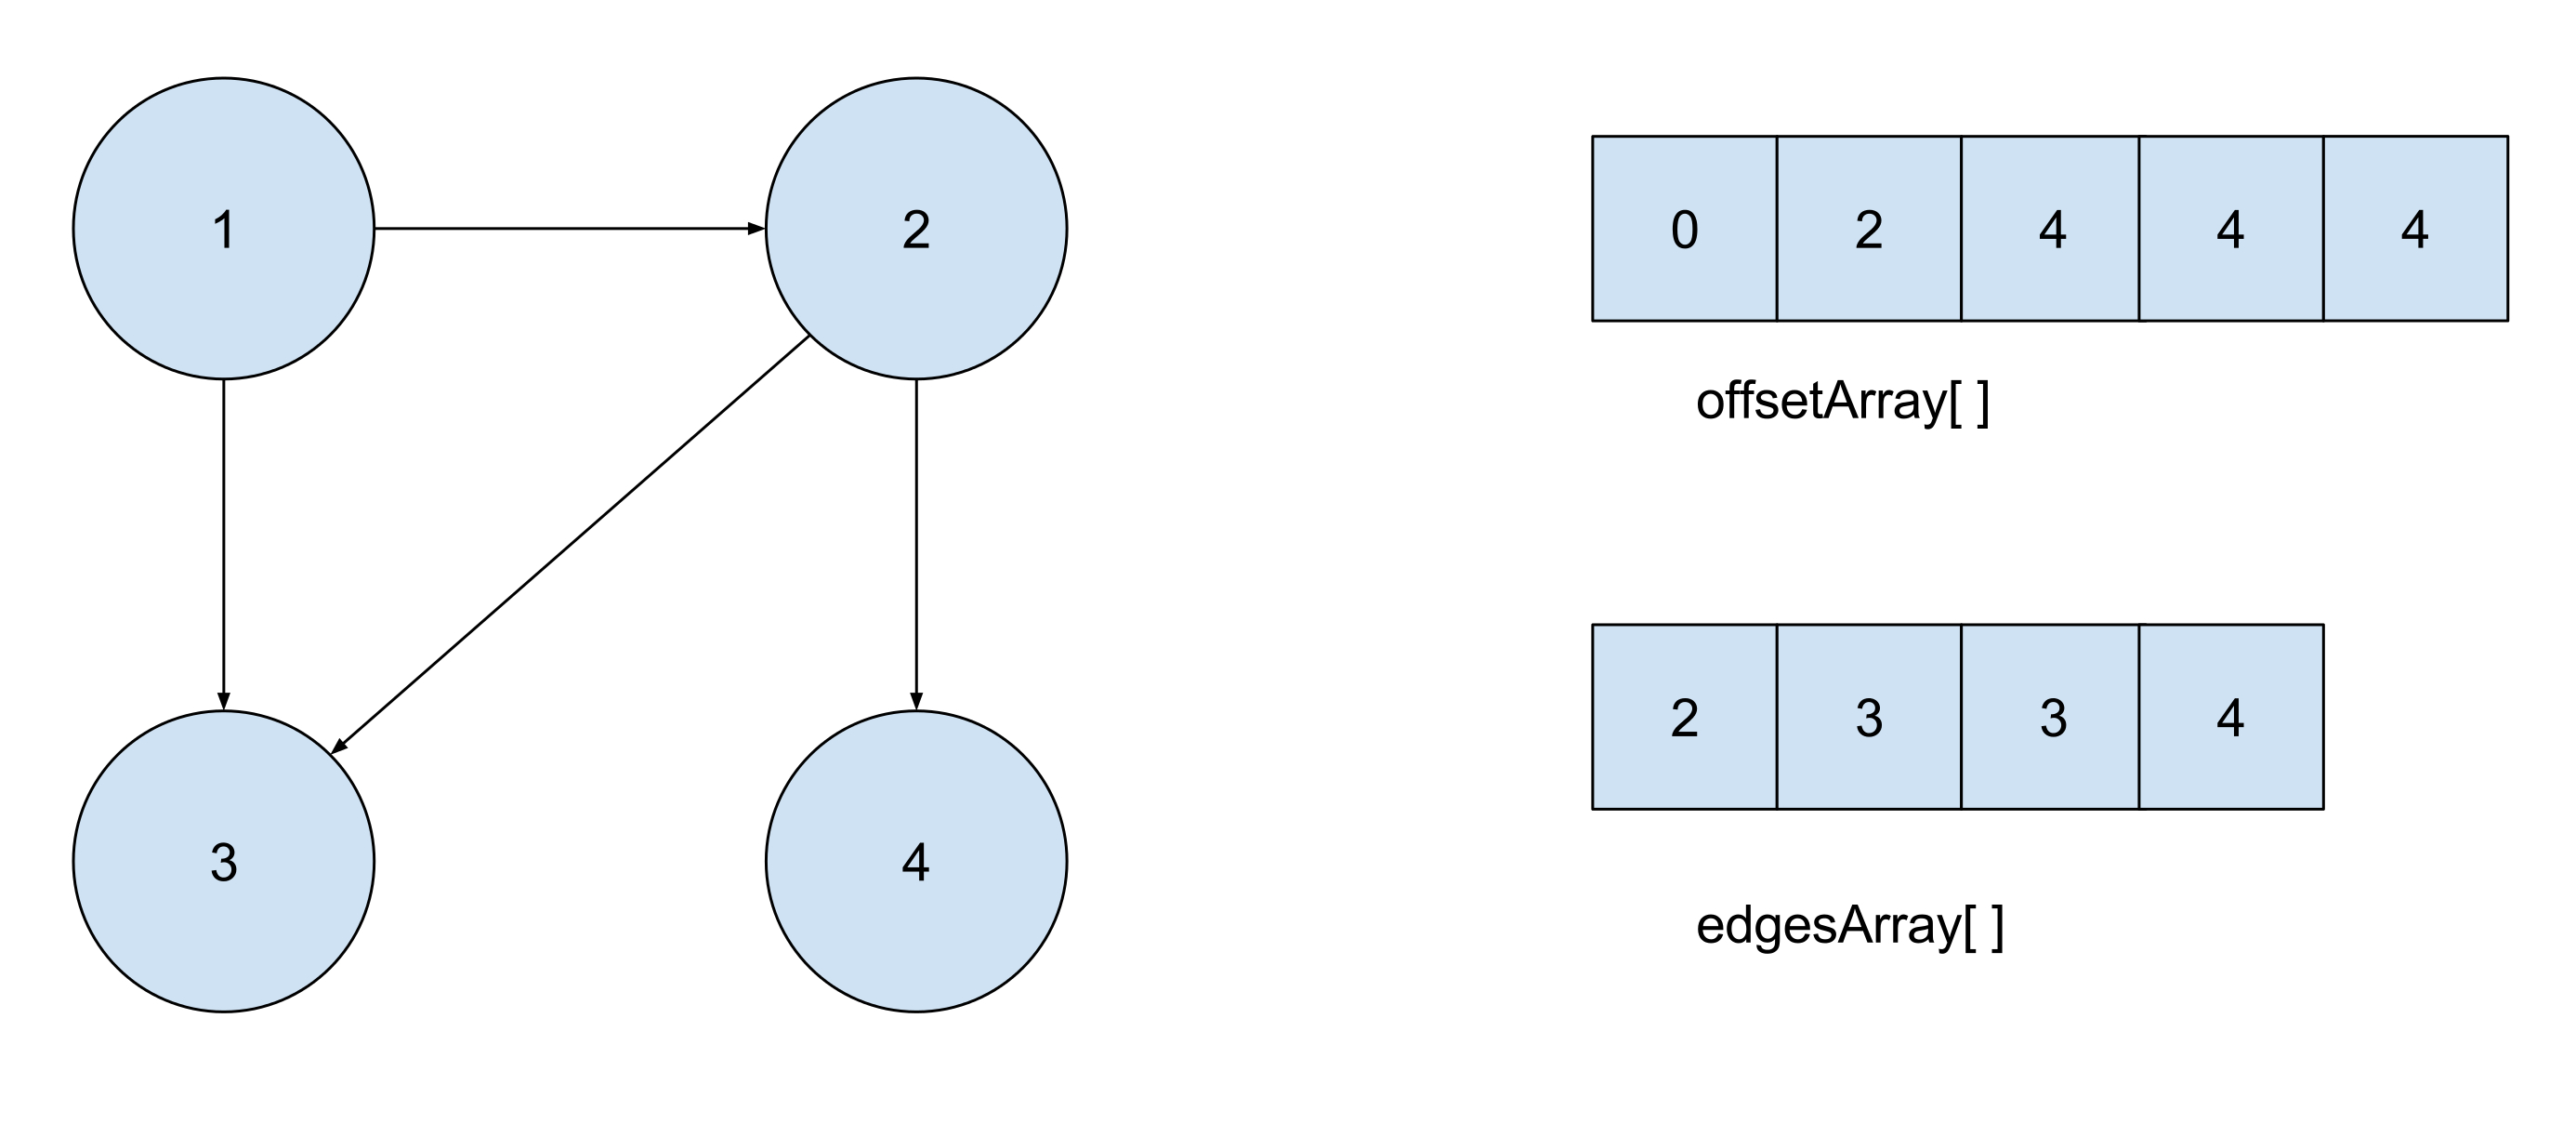
\includegraphics[width=\textwidth,scale=0.6,keepaspectratio=true]{csrdirected.jpg}
    \caption{
       The Directed Graph from \ref{table:1} and its CSR
    }
    \label{fig:csrd}
\end{figure}

Consider the undirected graph with $n=4$ and $m=3$ as given in the table \ref{table:2}. Its corresponding CSR is given in the figure \ref{fig:csru} and its UCSR is given in the figure \ref{fig:csrun}. Note that the \verb+edgesArray[]+ has $2m = 6$ elements in the UCSR.

\begin{table}[h!]
\centering
\begin{tabular}{||c|c||} 
 \hline
 Incident Node & Incident Node \\ [0.5ex] 
 \hline\hline
 1 & 2\\
 \hline
 1 & 4\\
 \hline
 2 & 3\\
 \hline
\end{tabular}
\caption{An Undirected Graph with $n=4$ and $m=3$}
\label{table:2}
\end{table}

\begin{figure}[h]
    \centering
    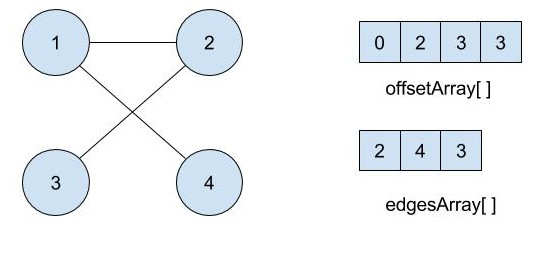
\includegraphics[width=\textwidth,scale=0.6,keepaspectratio=true]{csrundirected.jpg}
    \caption{
        The Undirected Graph from \ref{table:2} and its CSR
    }
    \label{fig:csru}
\end{figure}
\begin{figure}[h]
    \centering
    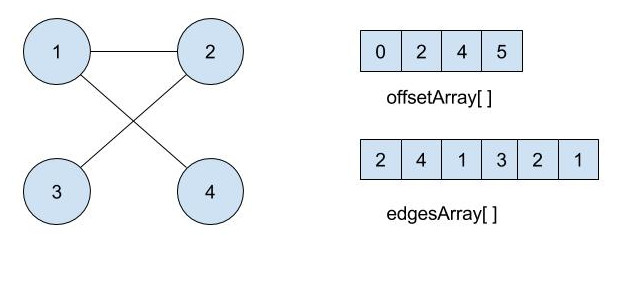
\includegraphics[width=\textwidth,scale=0.6,keepaspectratio=true]{csrundirectednew.jpg}
    \caption{
        The Undirected Graph from \ref{table:2} and its UCSR
    }
    \label{fig:csrun}
\end{figure}
\subsection{RANDCOLOUR: Random Colouring And Conflict Resolution}
We started with a random colouring and conflict resolution based algorithm which we call \verb+RANDCOLOUR+. This is an algorithm pertaining to the category covered by Algorithm \ref{SpecColouring}. We first speculate the colours randomly and then find the conflicts on the GPU, both of which are done in parallel. Then we resolve the conflicts sequentially on the CPU. As we know, a graph $G(V,E)$ with maximum degree $\Delta$ can be coloured with atmost $\Delta+1$ colours, RANDCOLOUR is an attempt at a fast $\Delta+1$ colouring using GPU. \verb+RANDCOLOUR+ algorithm produces a worst colour quality of $\Delta+1$ and was aimed at a fast colouring compromising colour quality in the process.

\begin{algorithm}
\caption{RANDCOLOUR}\label{randcolour}
\begin{algorithmic}[1]
\Procedure{RandomColouring(G(V,E))}{}
\State $\textit{Initialization}$
\BState \emph{GPU (Speculation)}:
\State $\textit{Initialize MaxDegree}$ \Comment{Found in parallel on GPU} \label{8.4}
\For {$each \: v \in V$}\Comment{Done in parallel by |V| threads} \label{8.5}
\State $colour[v] \gets CURAND(MaxDegree+1)+1$\Comment{RAND on GPU} \label{8.6}
\EndFor
\BState \emph{GPU (Conflict Detection)}:
\State $\textit{conflictSet} \gets \phi$ \label{8.8}
\For{$each \: v \in V$} \Comment{Done in parallel}
\For{$each \: u \in V$ such that $u$ and $v$ are adjacent}
\If{$colour[v] = colour[u]$}
\State $\textit{conflictSet} \gets \textit{conflictSet} \cup \{min(v,u)\}$ \label{8.12}
\EndIf
\EndFor
\EndFor
\BState \emph{CPU (Conflict Resolution)}:
\For {$each \: v \in \textit{conflictSet}$} \label{8.14}
\State $colour[v] \gets \textit{A colour by some greedy colouring algorithm}$ \label{8.15}
\EndFor
\EndProcedure
\end{algorithmic}
\end{algorithm}

The scheme is given in Algorithm \ref{randcolour}. First we find $\Delta$, the maximum degree of the graph (Line \ref{8.4}). This task can be done in parallel on the GPU. With UCSR of the graph, the degree of a vertex $i+1$ is given by \verb|offsetArray[i+1]|$-$\verb+offsetArray[i]+. Once we have $\Delta$, we use \verb+cuRAND+ library \citep{nVidia:cuRAND}, which generates random numbers really fast using CUDA capable GPUs, to colour the graph with random integers ranging from 1 to $\Delta+1$ (Lines \ref{8.5} and \ref{8.6}). Once this colouring is over, we try to find out the conflicts that were inflicted. This can be done in parallel on the GPU too (Lines \ref{8.8} to \ref{8.12}). We mark all the conflicts and then resolve them on the CPU using a greedy approach (Lines \ref{8.14} and \ref{8.15}).

\subsection{MINMAXCOLOUR: Maximal VIS And Colouring}
We then tried a version of the algorithm put forward by \citet{Jones:1993:PGC:153109.153119} which uses some of the suggestions by \citet{cohenefficient}. As discussed earlier, the algorithm by \citet{Jones:1993:PGC:153109.153119} is based on the category covered by Algorithm \ref{VISColouring}. So, here, we try to find Maximal Vertex Independent Sets and then colour them in parallel. 
\subsubsection{Improvements}
\begin{itemize}
\item The original version uses a \verb+Max+ approach for finding a Maximal Vertex Independent Set. A \verb+Min+ approach also gives us a Maximal Vertex Independent Set which is mutually exclusive with the \verb+Max+ based set (except when a vertex doesn't have any adjacent vertices; discussed in the next point). So, we find two Maximal Vertex Independent Sets in each iteration, one based on \verb+Max+ approach and the other on \verb+Min+ approach. Then, we colour both sets with two different colours in each iteration. This way we get to speed up the colouring by reducing the number of iterations required. 
\item Conflicts can arise when two neighbouring vertices have the same random number allotted to them. That same random number could be a neighbourhood minimum or maximum in which case we have multiple candidates for the \verb+Max+ set or \verb+Min+ set from the same neighbourhood. If a vertex doesn't have any neighbours, it can possibly be added to the  \verb+Max+ set as well as \verb+Min+ set. To avoid conflicts between the \verb+Max+ based set and \verb+Min+ based set in each iteration, we follow a set of conventions as follows:
\begin{itemize}
\item In each iteration, the \verb+Max+ based set takes the smaller of the two colour numbers allowed in that iteration.
\item If two neighbours have the same random number allotted to them, the vertex with a smaller index has higher precedence for \verb+Max+ set.
\item If two neighbours have the same random number allotted to them, the vertex with a higher index has higher precedence for \verb+Min+ set.
\item If a vertex doesn't have any neighbours, it is considered a local maxima and is added to \verb+Max+ set. This is because \verb+Max+ sets get a lower colour number compared to \verb+Min+ sets in an iteration as discussed earlier. 
\end{itemize}
\end{itemize}

The scheme for this is given in Algorithms \ref{MinMaxSet} and \ref{MinMaxAlgo}. In Algorithm \ref{MinMaxSet}, we have the Min-Max Maximal Independent Set algorithm which is an improved version of \citet{Luby:1985:SPA:22145.22146}. The two inner for loops in the algorithm at Line \ref{9.7} and Line \ref{9.17} can be merged together using some conditionals. We find two maximal sets in each iteration. If a vertex doesn't have any neighbours, it will be a part of both the \verb+Min+ set and the \verb+Max+ set. In Line \ref{9.26}, we make sure such vertices go to only the Max set. In the colouring part, in each iteration, we colour the Max set with a colour $c$ (Lines \ref{10.8} and \ref{10.9}) and the Min set with $c+1$ (Lines \ref{10.10} and \ref{10.11}). The algorithm is iterated until there are no vertices left to colour (Line \ref{10.6}). The maximal sets are found in parallel and they can be coloured in the same kernel call.  

\begin{algorithm}
\caption{Min-Max Maximal Vertex Independent Sets}\label{MinMaxSet}
\begin{algorithmic}[1]
\Procedure{MinMaxMaximalSet(G(V,E))}{}
\State $\textit{Initialization}$\Comment{randomNumber[] is initialized only once}
\State $MinS \gets \phi$
\State $MaxS \gets \phi$
\For {$each \: v \in V$}\Comment{Done in parallel}
\State $MaxS \gets MaxS \cup \{v\}$
\For {$each \: u \in V$ such that $u$ is adjacent to $v$}\label{9.7}
\If{$\textit{randomNumber}[u] > \textit{randomNumber}[v]$}
\State $S \gets S \: \textbackslash \: v$
\State $\textit{break}$
\Else \If{$\textit{randomNumber}[u] = \textit{randomNumber}[v]$} 
\If{$u>v$} 
\State $S \gets S \: \textbackslash \: v$
\State $\textit{break}$
\EndIf
\EndIf
\EndIf
\EndFor
\State $MinS \gets MinS \cup \{v\}$
\For {$each \: u \in V$ such that $u$ is adjacent to $v$}\label{9.17}
\If{$\textit{randomNumber}[u] < \textit{randomNumber}[v]$}
\State $S \gets S \: \textbackslash \: v$
\State $\textit{break}$
\Else \If{$\textit{randomNumber}[u] = \textit{randomNumber}[v]$} 
\If{$u<v$} 
\State $S \gets S \: \textbackslash \: v$
\State $\textit{break}$
\EndIf
\EndIf
\EndIf
\EndFor
\EndFor
\State $MinS \gets MinS \: \textbackslash \: MaxS$ \label{9.26}
\State $\textit{return} \: MaxS, MinS$ 
\EndProcedure
\end{algorithmic}
\end{algorithm}

\begin{algorithm}
\caption{MINMAXCOLOUR}\label{MinMaxAlgo}
\begin{algorithmic}[1]
\Procedure{MinMaxColouring(G(V,E))}{}
\State $\textit{Initialization}$
\State $n \gets 0$
\State $currentColour \gets 1$
\State $graphSize \gets |V|$
\While{$n \neq graphSize$} \Comment{Or $V \neq \phi$} \label{10.6}
\State $MaxS, MinS \gets $\verb+MinMaxMaximalSet(V,E)+
\For {$each \: v \in MaxS$}\Comment{Done in parallel} \label{10.8}
\State $colour[v] \gets currentColour$ \label{10.9}
\EndFor
\For {$each \: v \in MinS$}\Comment{Done in parallel} \label{10.10}
\State $colour[v] \gets currentColour+1$ \label{10.11}
\EndFor
\State $currentColour \gets currentColour+2$
\State $n \gets n+|MaxS|+|MinS|$
\State $V \gets V \: \textbackslash \: MaxS$
\State $V \gets V \: \textbackslash \: MinS$
\EndWhile
\EndProcedure
\end{algorithmic}
\end{algorithm}

The Maximal VIS based algorithm might be a little more time consuming as it employs an iterative approach, but should produce better colour quality. The main reason why this approach was our choice is because the entire process happens in parallel here, that is there is no sequential colouring component. As we use GPU, we try to maximize the use of the massive parallelism GPUs offer.
\chapter{PARALLEL GRAPH COLOURING: INCREMENTAL}
\section{Why Incremental?}
Graphs are being used in a varied lot of applications these days. Graphs are ever more important and ever growing. Practical graphs like social networks graphs, communication networks graphs are inherently dynamic. Most of them keep on changing. Edges and Vertices get added and deleted every now and then. It is not a great idea to run a computationally intensive algorithm again on a graph just because a few thousands (a small fraction compared to total graph size) of edges are added to it. Thus incremental approaches are very important so as to save on computation and time.

\section{Handling a Growing Graph}
So, with incremental graph colouring, we are accommodating additions of vertices and edges. We assume without any loss of functionality that no new vertices are added. Only edges are added. This is easy to see as adding a new vertex (with some edges incident on it) is equivalent to adding edges to a vertex with zero degree. As long as we have an idea about the upper bound on the number of vertices through the applications of the graph, we should be fine. 

Through the additions of edges, the \verb+offsetArray[]+ of UCSR doesn't grow in size. But the size of \verb+edgesArray[]+ will grow. So, we should have a reasonable upper bound on the number of edges that can be incident on each vertex. We can set the extra \verb+edgesArray[]+ elements to zero initially. When an edge is added, the new edge's information can be added to the \verb+edgesArray[]+ at these elements which are set to zero.

\section{The Two Thread Incremental Model}
We assume we have a graph which is already coloured using one of the algorithms, in our case Algorithm \ref{MinMaxAlgo} from last chapter, on the GPU. We also assume that we have the UCSR graph already residing on the GPU memory. 

In the incremental model, when an edge is added, only two vertices are immediately affected. The vertices on which the added edge is incident. If those two vertices have different colours, already, we assume they were coloured optimally by the main algorithm already and leave those two vertices be with their existing colours. If those two vertices have the same colour, then we have a conflict on the addition of the new edge. We are concerned with only those two vertices for the immediate task of resolving the conflict.

We introduce an algorithm called The Two Thread Incremental Model to deal with recolouring the graph. This model makes use of only two threads, each thread for each of the two vertices in conflict, as our immediate objective is to remove the conflict. But, in our model, while removing the conflict, we try to optimize the colours of those two vertices and thus locally maximizing the colour quality. It follows that when the colours of the two vertices are changed in a locally optimized way, there could be positive changes in the other parts of the graph. We will deal with this later in the propagation part.

\begin{algorithm}
\caption{The Two Thread Incremental Model}\label{twoThreadIncremental}
\begin{algorithmic}[1]
\Procedure{TwoThreadIncrementalColouring(G(V,E), edge)}{}
\State $\textit{Initialization}$
\State \textit{Let uv be the newly added edge}
\State \textit{Thread 0 represents u and thread 1 represents v}
\State $\textit{Add the new edge information to the UCSR}$\Comment{Each thread add its neighbour}
\State \textit{synchronize}
\If{$colour[u] \neq colour[v]$}
\State \textit{return}
\EndIf
\For {$i \in \{u, v\}$} \Comment{In parallel by two threads}
\State $oldColour \gets colour[i]$
\State $possibleColour[threadId] \gets \textit{Smallest possible colour for i}$
\State $possibleColour2[threadId] \gets \textit{Second smallest possible colour for i}$
\State \textit{synchronize}

\If {$possibleColour[threadId]=possibleColour[1-threadId]$}

	\If {$possibleColour[threadId]<oldColour$}

		\If {$possibleColour2[threadId]<possibleColour2[1-threadId]$}
\BState \emph{Label 1}:
			\If {$possibleColour2[threadId]<oldColour$}
				\State $colour[i] \gets possibleColour2[threadId]$
			\EndIf

		\Else
			\If {$possibleColour2[threadId] = possibleColour2[1-threadId]$}
\BState \emph{Label 2}:
				\If {\textit{threadId}$=0$}
					\State $colour[i] \gets possibleColour[threadId]$
				\Else
\BState \emph{Label 3}:
					\If {$possibleColour2[threadId]<colour[i]$}
						\State $colour[i] \gets possibleColour2[threadId]$
					\EndIf
				\EndIf

			\Else
\BState \emph{Label 4}:	
				\State $colour[i] \gets possibleColour[threadId]$
			\EndIf

		\EndIf

\Else
\BState \emph{Label 5}:
\If {\textit{threadId}$=1$}
\State $colour[i] \gets possibleColour[threadId]$
\EndIf
\EndIf
\Else
\BState \emph{Label 6}:
\If {$possibleColour[threadId]<oldColour$}
\State $colour[i] \gets possibleColour[threadId]$
\Else
\BState \emph{Label 7}:
\If {$possibleColour[threadId]<possibleColour[1-threadId]$}
\State $colour[i] \gets possibleColour[threadId]$
\EndIf
\EndIf
\EndIf
\EndFor
\EndProcedure
\end{algorithmic}
\end{algorithm}

Our Two Thread Incremental Model is explained in Algorithm \ref{twoThreadIncremental}. From the structure of the problem and our algorithm, it is clear that we actually need only two threads to deal with locally maximizing the colour quality at the region of edge addition. As we have the graph already on the GPU memory, we don't have an issue with memory latency, the biggest hurdle with GPGPU.

This algorithm is meant for addition of a single edge. Two threads are spawned to run the algorithm. Each thread takes charge of one of the vertices on which the new edge is incident. In our algorithm, we assume \textit{uv} is the added edge and \textit{Thread 0} is in charge of \textit{u} and \textit{Thread 1} in charge of \textit{v}. Initially, each thread modifies its portion of the UCSR to accommodate the newly added edge. Then they check if the current colouring of \textit{u} and \textit{v} are the same. If not, we are through.

If the current colouring of \textit{u} and \textit{v} are the same, we first try to find out the least colour they can assume considering their neighbourhood in a greedy fashion. This new colouring cannot be their existing colour, as both of them have each other as a neighbour now. Let the current colouring be called \textit{p}. Let the newly found least possible colour for each of them be \textit{x} and \textit{y}. Now, we have $x \neq p$ and $y \neq p$. In the case of $x=y$, let $a$ and $b$  be the least colour greater than $x$ and $y$ respectively that \textit{u} and \textit{v} can take respectively in a greedy fashion. We have many cases that can arise in most of which $u, x, a$ and $v, y, b$ are interchangeable with no side effects. These cases and the actions required are tabulated in Table \ref{table:3}. 

\begin{table}[h]
\centering
\begin{tabular}{||c|c|c|c||} 
 \hline
 No & Case & Action & Label No. in Algorithm \\ [0.5ex] 
 \hline\hline
1 & $x=y < p; \: a=b<p$ & $colour[u]=x; \: colour[v]=b$ & 2, 3 \\
\hline
2 & $x=y < p; \: p<a=b$ & $colour[u]=x$ & 2 \\
\hline
3 & $x=y < p; \: a<b; \: a<p$ & $colour[u]=a; \: colour[v]=y$ & 1, 4 \\
\hline
4 & $x=y < p; \: a<b; \: p<a$ & $colour[v]=y$ & 4 \\
\hline
5 & $p < x=y$ & $colour[v]=y$ & 5\\
\hline
6 & $x \neq y; \: x < y < p$ & $colour[u]=x; \: colour[v]=y$ & 6\\
\hline
7 & $x \neq y; \: x < p < y$ & $colour[u]=x$ & 6\\
\hline
8 & $x \neq y; \: p < x < y$ & $colour[u]=x$& 7\\
\hline
\end{tabular}
\caption{Two Threads Model: Different Cases}
\label{table:3}
\end{table}

Each of the cases given in the table \ref{table:3} are explained using examples in the figures \ref{fig:case1}, \ref{fig:case2}, \ref{fig:case3}, \ref{fig:case4}, \ref{fig:case5}, \ref{fig:case6}, \ref{fig:case7} and \ref{fig:case8}.

\begin{figure}[h]
    \centering
    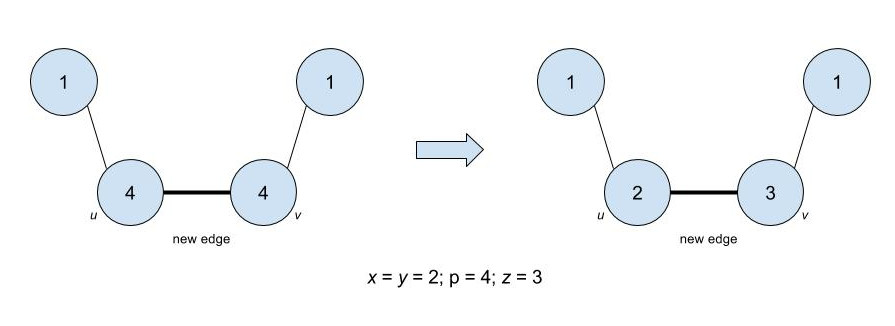
\includegraphics[width=\textwidth,keepaspectratio=true]{case1.jpg}
    \caption{
        \textbf{Case 1:} $x=y < p; \: a=b<p$
    }
    \label{fig:case1}
\end{figure}

\begin{figure}[h]
    \centering
    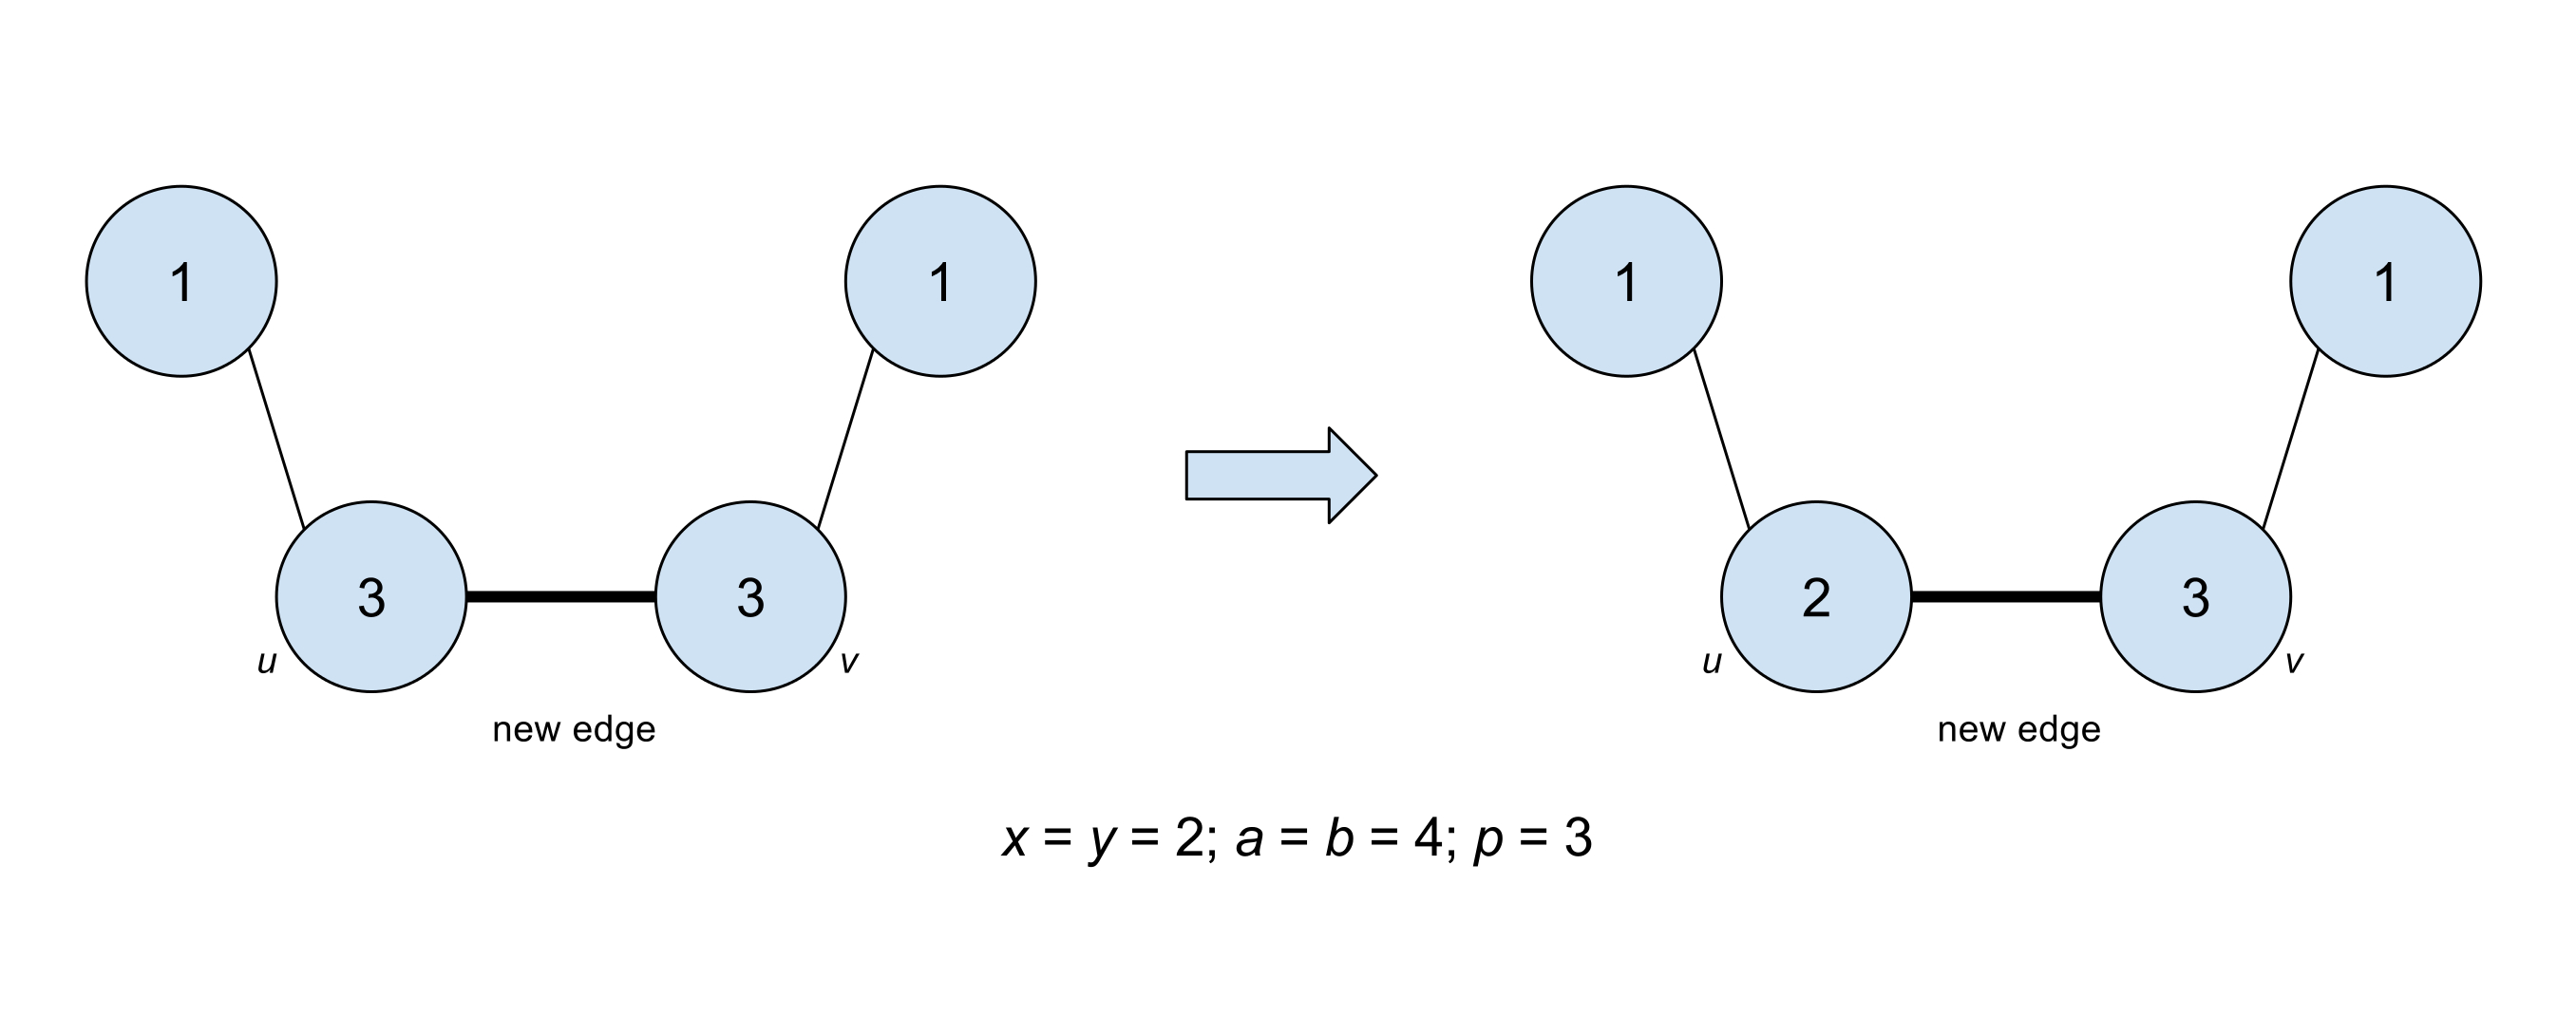
\includegraphics[width=\textwidth,keepaspectratio=true]{case2.jpg}
    \caption{
        \textbf{Case 2:} $x=y < p; \: p<a=b$
    }
    \label{fig:case2}
\end{figure}

\begin{figure}[h]
    \centering
    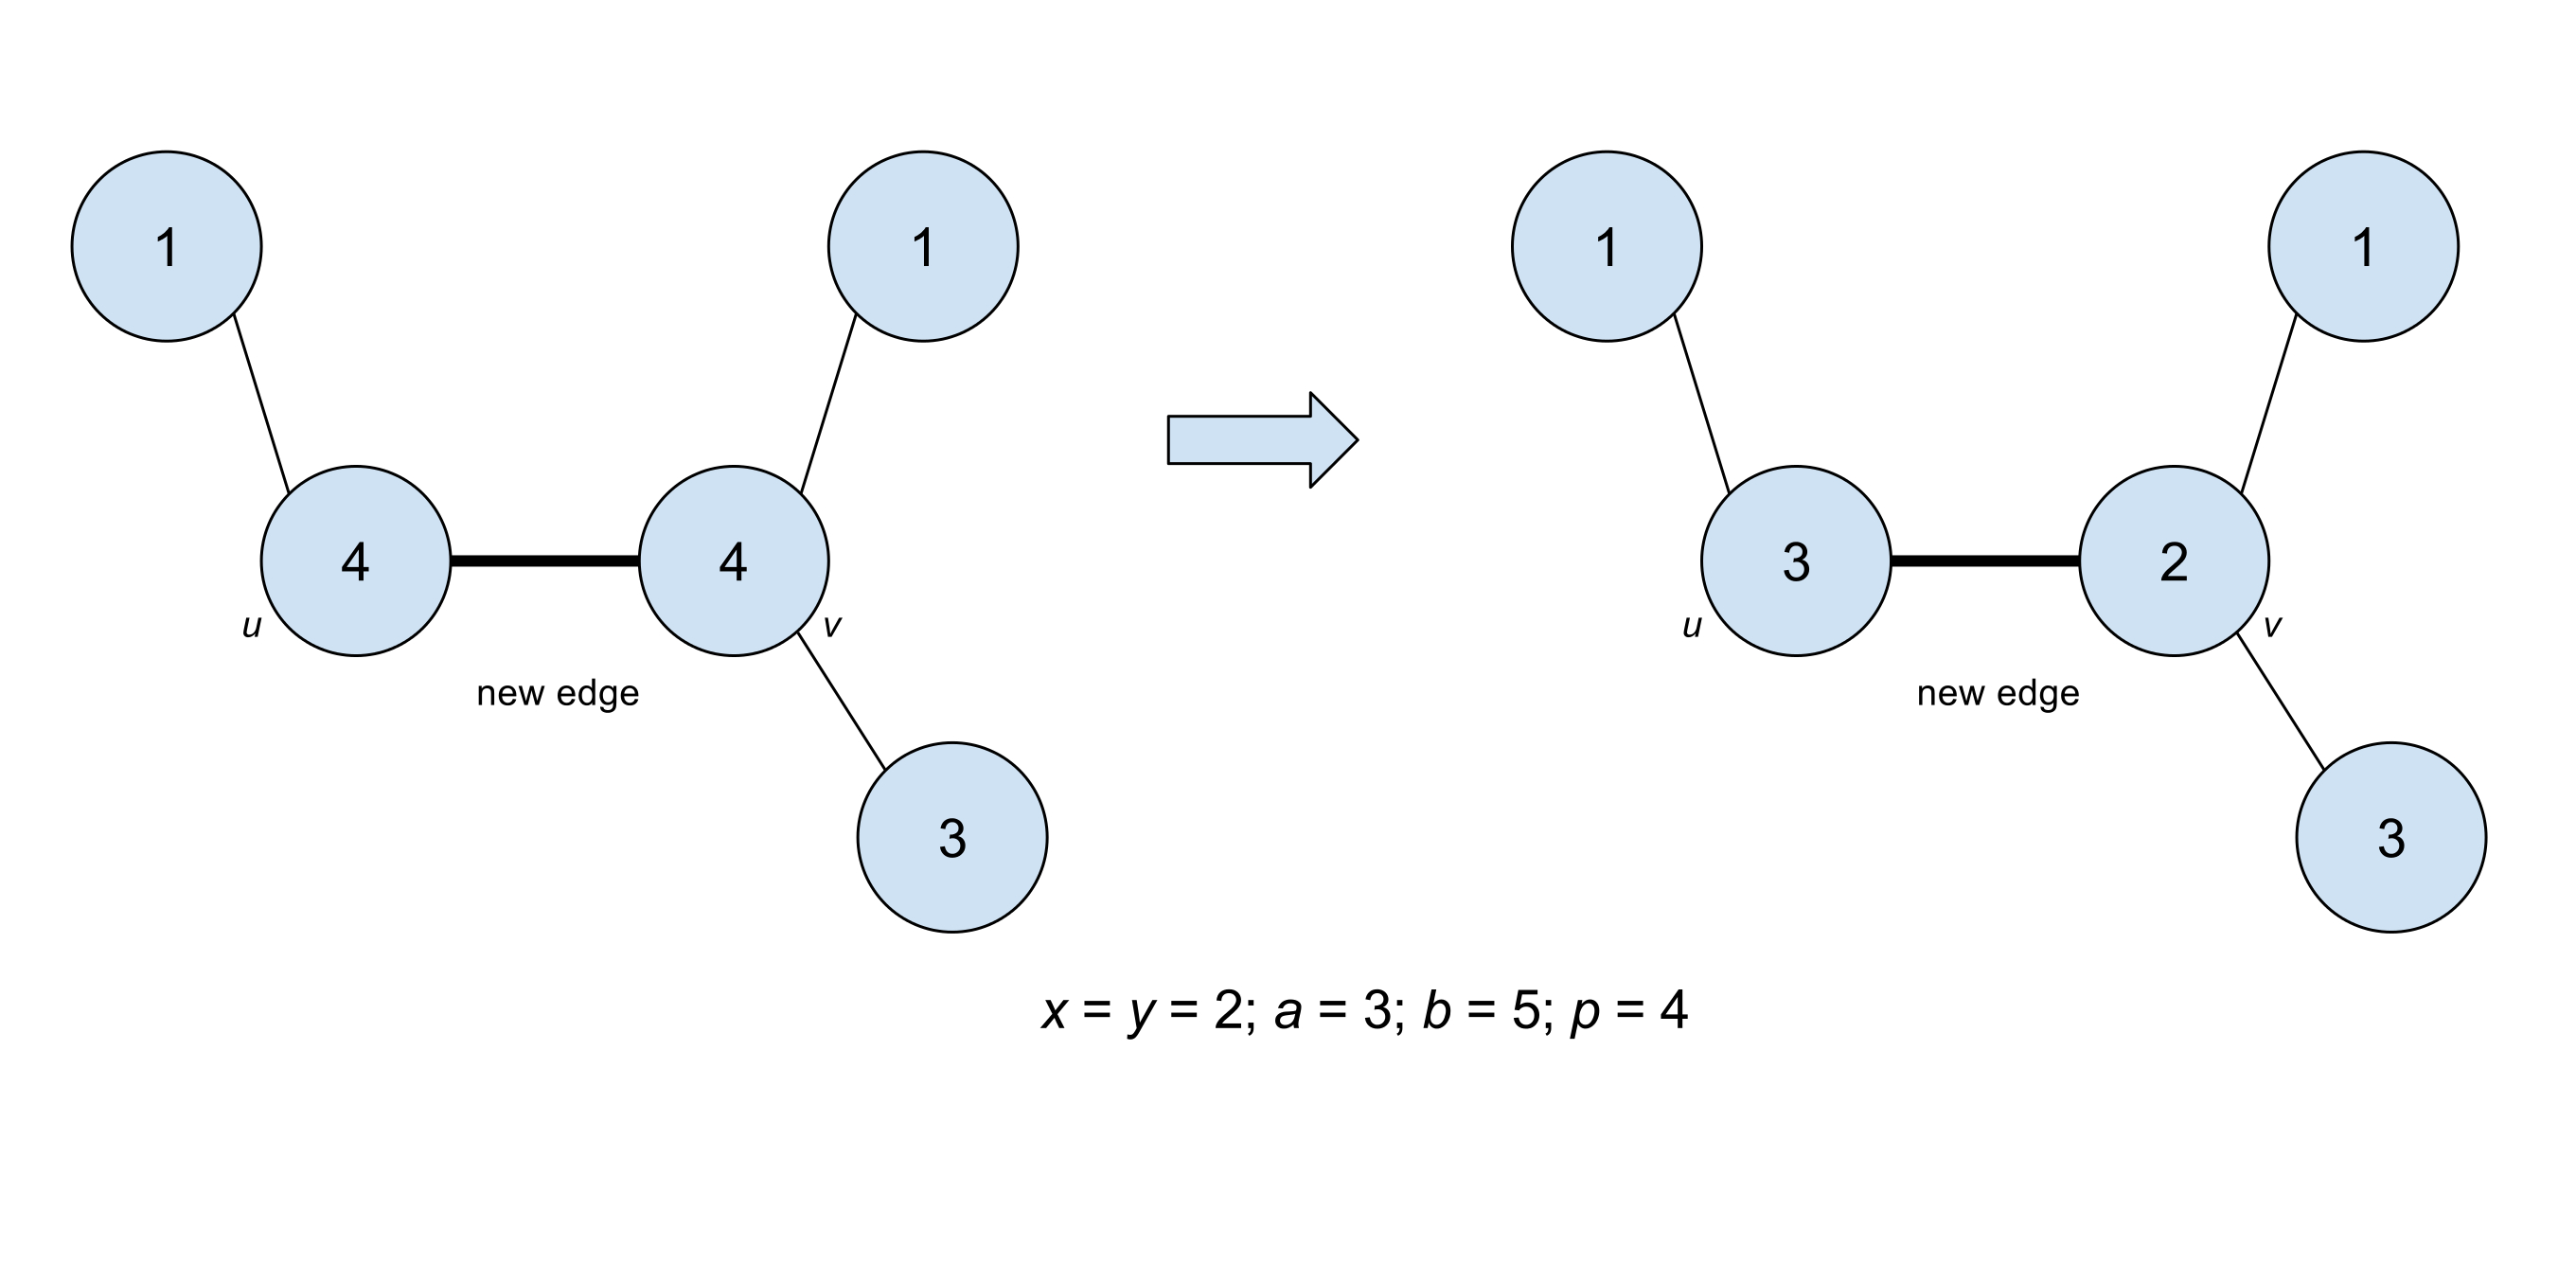
\includegraphics[width=\textwidth,keepaspectratio=true]{case3.jpg}
    \caption{
        \textbf{Case 3:} $x=y < p; \: a<b; \: a<p$
    }
    \label{fig:case3}
\end{figure}

\begin{figure}[h]
    \centering
    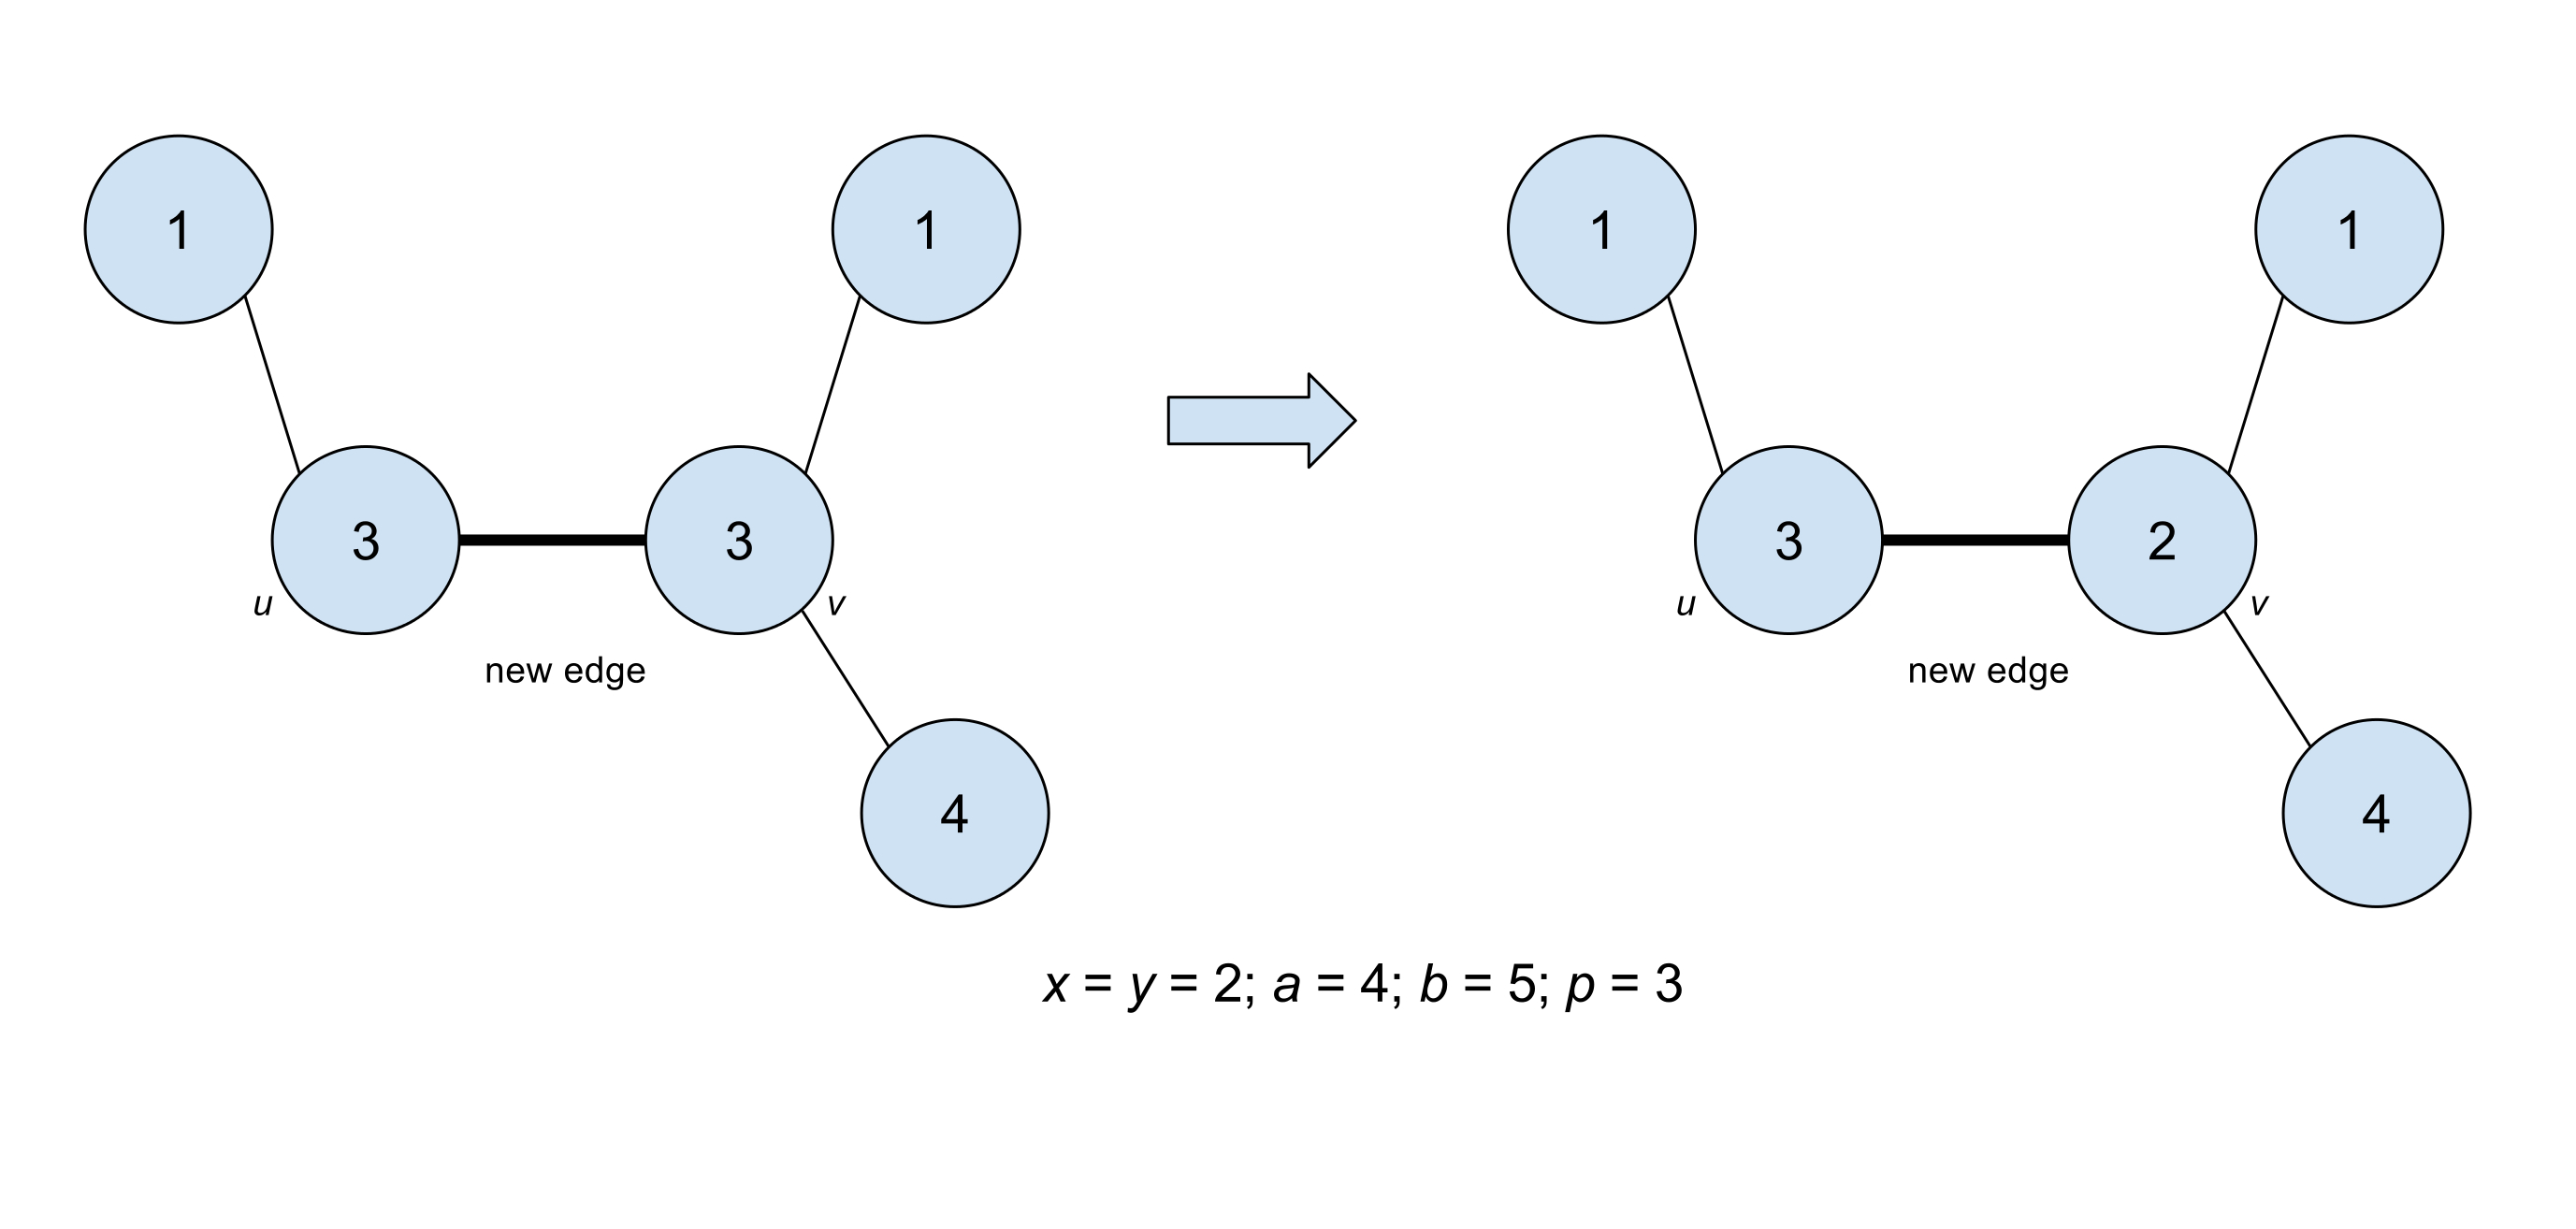
\includegraphics[width=\textwidth,keepaspectratio=true]{case4.jpg}
    \caption{
        \textbf{Case 4:} $x=y < p; \: a<b; \: p<a$
    }
    \label{fig:case4}
\end{figure}

\begin{figure}[h]
    \centering
    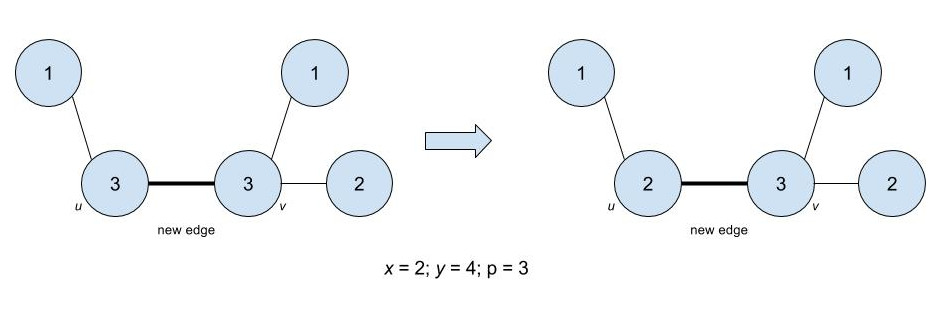
\includegraphics[width=\textwidth,keepaspectratio=true]{case5.jpg}
    \caption{
        \textbf{Case 5:} $p < x=y$
    }
    \label{fig:case5}
\end{figure}

\begin{figure}[h]
    \centering
    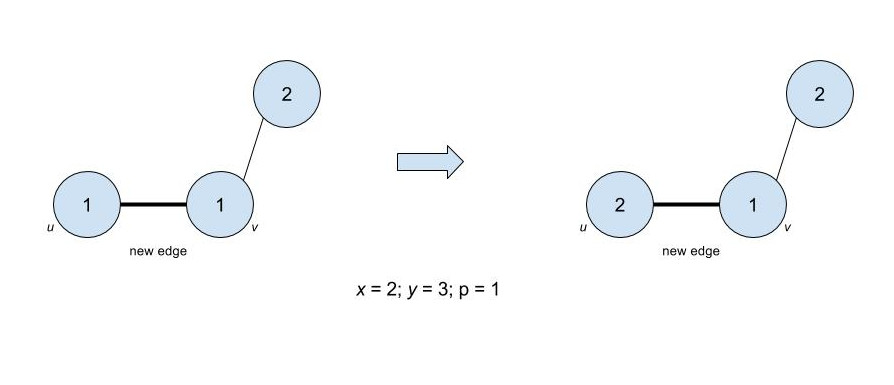
\includegraphics[width=\textwidth,keepaspectratio=true]{case6.jpg}
    \caption{
        \textbf{Case 6:} $x \neq y; \: x < y < p$
    }
    \label{fig:case6}
\end{figure}

\begin{figure}[h]
    \centering
    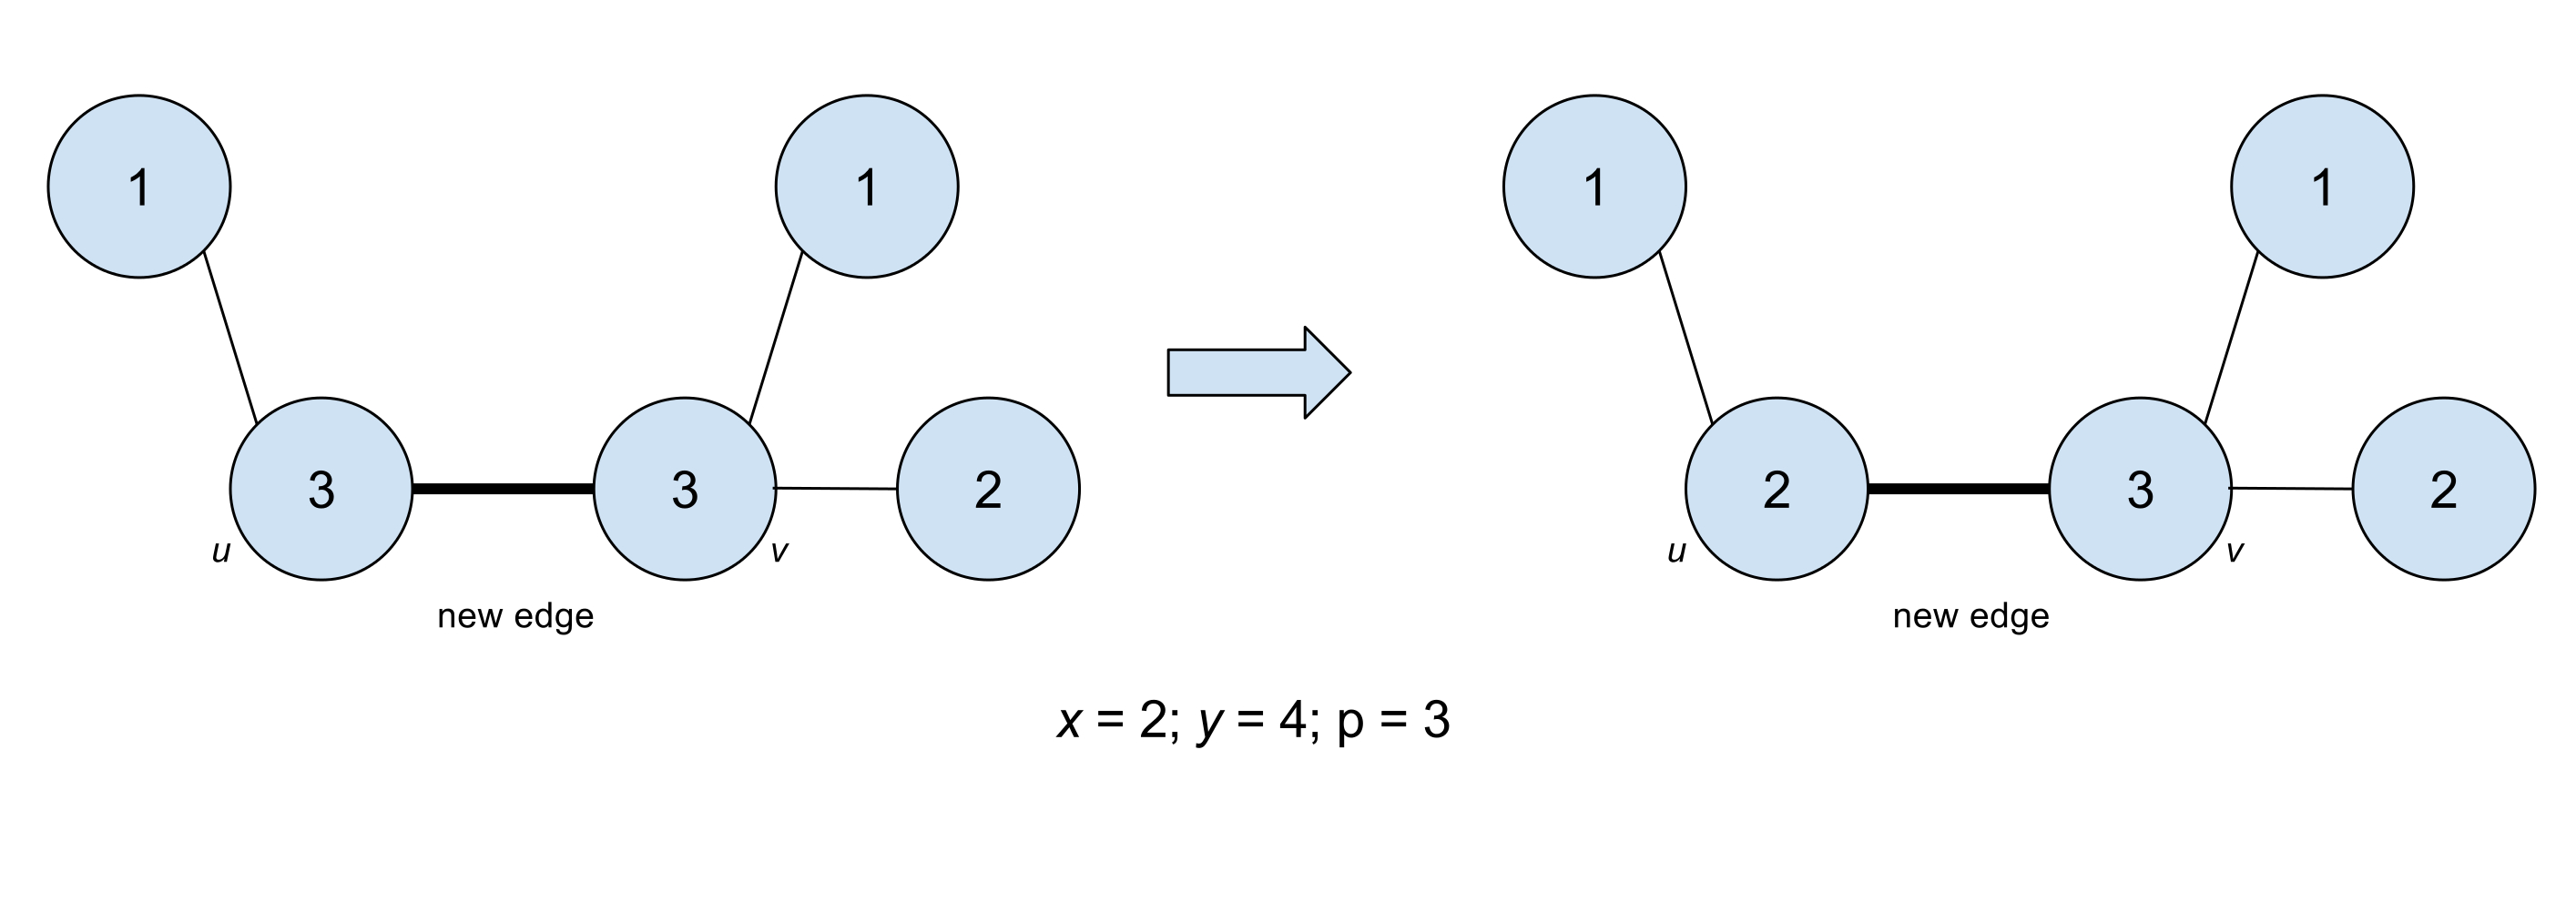
\includegraphics[width=\textwidth,keepaspectratio=true]{case7.jpg}
    \caption{
        \textbf{Case 7:} $x \neq y; \: x < p < y$
    }
    \label{fig:case7}
\end{figure}

\begin{figure}[h]
    \centering
    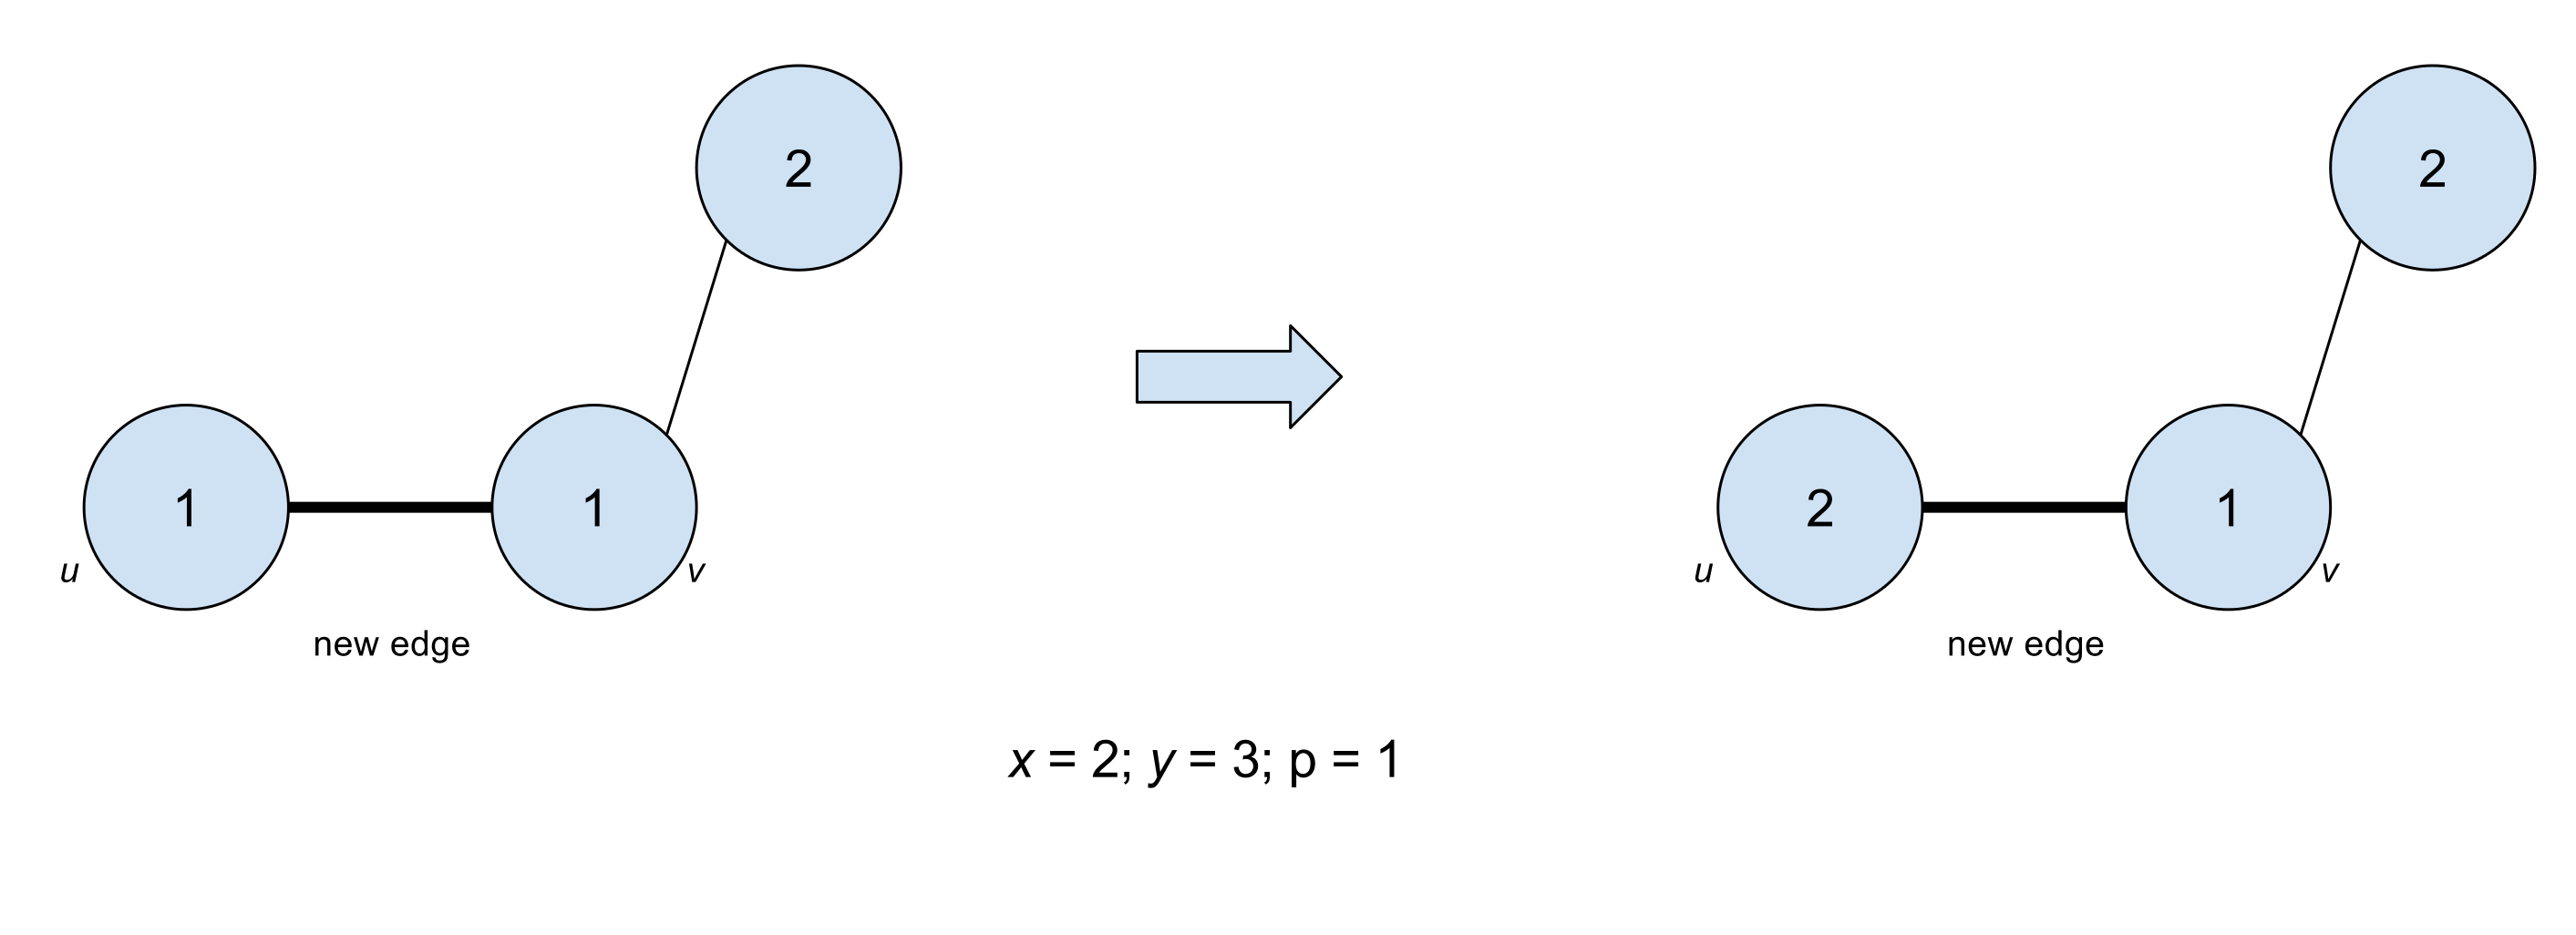
\includegraphics[width=\textwidth,keepaspectratio=true]{case8.jpg}
    \caption{
        \textbf{Case 8:} $x \neq y; \: p < x < y$ 
    }
    \label{fig:case8}
\end{figure}

\section{The Many Thread Incremental Model}
We have seen in The Two Thread Incremental Model in the last section and how it actually requires only two threads per addition of a new edge. As the graph is already on the GPU, we don't have much memory latency issues too. But then, GPUs are devices for massive parallelism. In this section, we will try to increase the parallelism involved in Incremental colouring.

As we have seen in the last session, we can handle a newly added edge with 2 threads. That is, if we colour on the go, we have to call a kernel with 2 threads each time we come across a new edge. To increase parallelism, we can try to club a bunch of new edges and process them together. But these edges shouldn't have any data races among them. So, we try to club edges which won't have any data races amongst them and process them all together in parallel. We call our new approach \textbf{The Many Thread Incremental Model} and it is explained in Algorithm \ref{manythread}.

According to our algorithm, we keep on taking new edges as inputs and add them to \verb+edgeSet+, as long as all the edges stored in our \verb+edgeSet+ are data race free. That is, there are no two edges which are incident on a common vertex. If a new edge added doesn't hold this true, we process the existing \verb+edgeSet+, all the edges processed in parallel with each edge getting two threads each, using \verb+TwoThreadIncrementalModel+ as discussed in the previous section. Once all the edges from \verb+edgeSet+ are processed, it is cleared and the new edge is added to it. Then it goes back to accepting more edges. 

New added edges can create conflicts. These conflicts will be resolved only after these edges are processed. So, it is not wise to wait for very long to club them with other edges for added parallelism. So, in our implementation, we have set a limit of 1024 edges as the maximum \verb+edgeSet+ size before it is forcibly processed.

\begin{algorithm}
\caption{The Many Thread Incremental Model}\label{manythread}
\begin{algorithmic}[1]
\Procedure{ManyThreadIncrementalColouring(G(V,E), edge)}{}
\State $\textit{Initialization}$
\State $\textit{edgeSet} \gets \phi$
\BState \emph{NewEdge}:
\State \textit{Take the new edge to be added, $\bar{e}$, as the input}
\State $\bar{u}, \bar{v} \gets \textit{endpoints of }\bar{e}$
\For {$each \: e \in edgeSet$}
\State $\textit{u, v} \gets \textit{endpoints of e}$

\State $setU \gets V \: \textbackslash \: adj(u)$\Comment adj(k) gives adjacent vertices of k
\State $setV \gets V \: \textbackslash \: adj(v)$
\State $setPermissible \gets setU \cap setV$

\If {$\bar{u} \not\in setPermissible \: OR \: \bar{v} \not\in setPermissible$}
\State // Done in parallel for all edges in the edgeSet
\State \verb+TwoThreadIncrementalColouring(G(V,E), edgeSet)+
\State $\textit{edgeSet} \gets \{\bar{e}\}$
\State \textit{goto NewEdge}
\EndIf
\EndFor
\State $\textit{edgeSet} \gets \textit{edgeSet} \cup \bar{e}$
\State \textit{goto NewEdge}
\EndProcedure
\end{algorithmic}
\end{algorithm}

\section{Propagation}
As discussed earlier, our algorithm tries improves the colouring locally at the end points of the new edge added. But, we consider only those two vertices. If any of them changes its colouring, it could have an effect on its adjacent vertices who could now probably improve their own colouring as they themselves might not be locally optimized. When they indeed change their colours, there could be scope for improvement in their neighbourhood. So, this has a ripple effect. The need for propagation and propagation itself is portrayed with the help of an example in the figure \ref{fig:propagation}.

\begin{figure}[h]
    \centering
    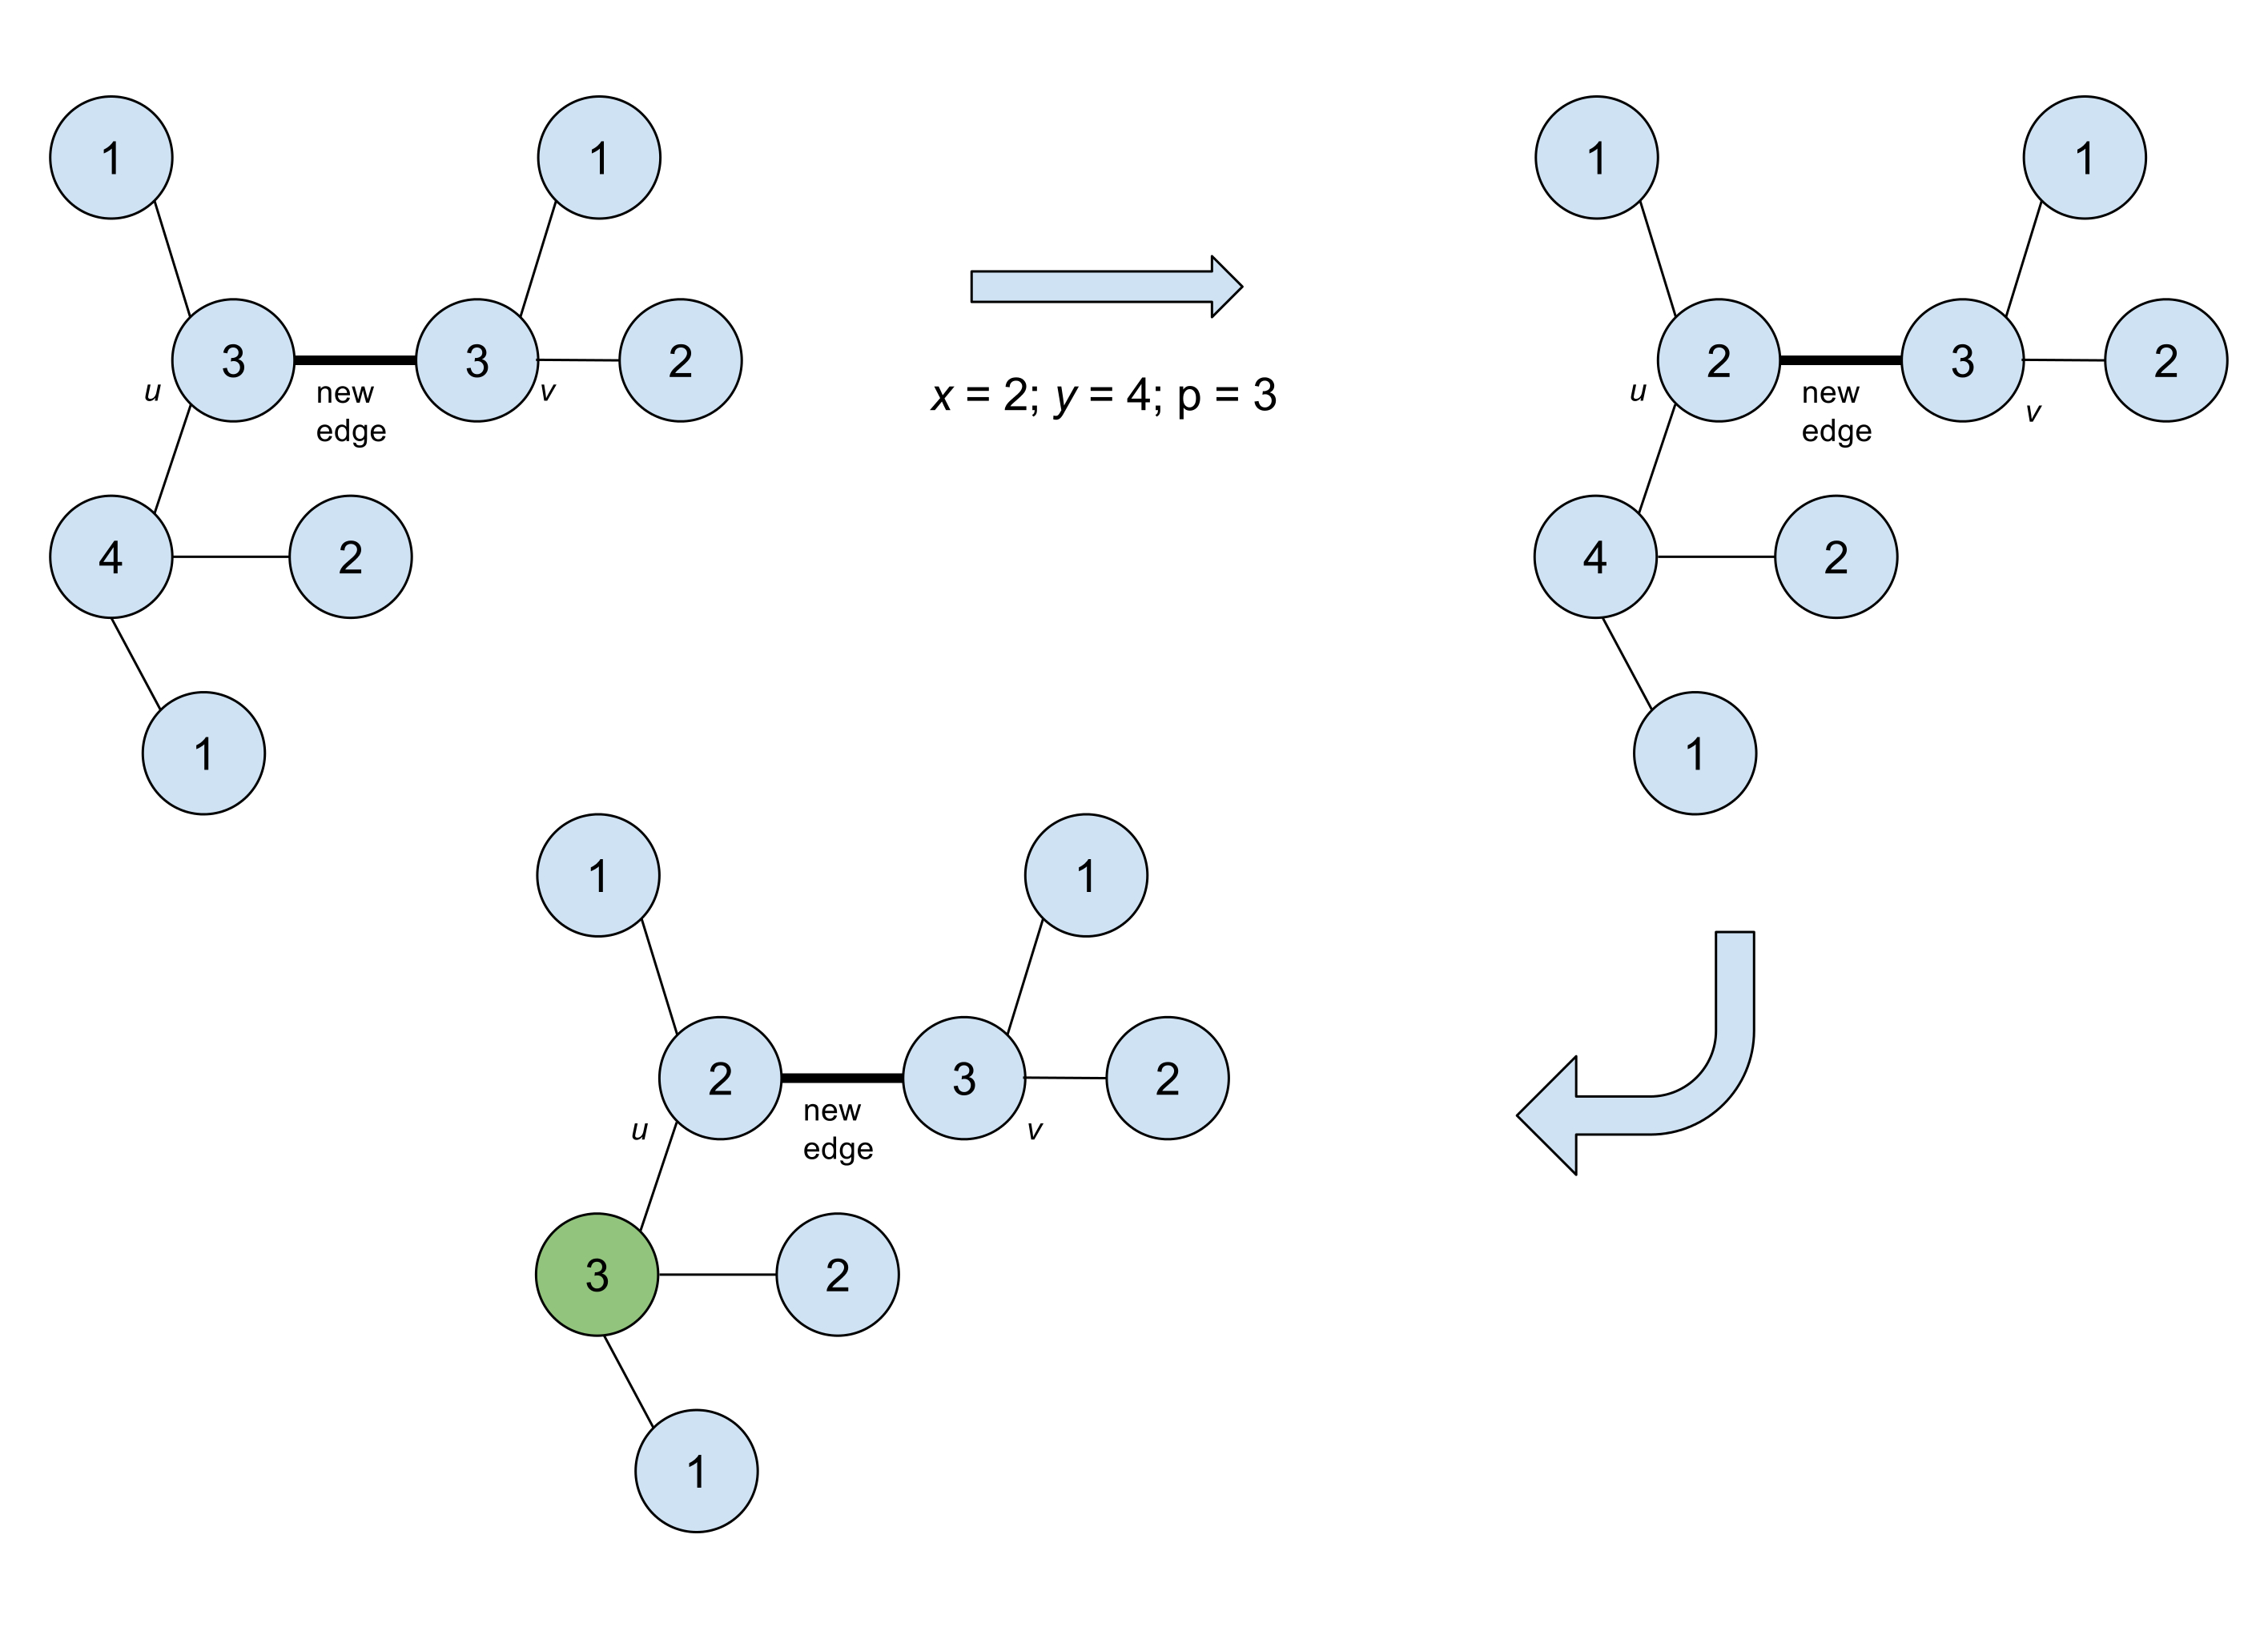
\includegraphics[width=\textwidth,keepaspectratio=true]{propagation.jpg}
    \caption{
        1-step propagation after adding a new edge and processing it. 
    }
    \label{fig:propagation}
\end{figure}

Though our locally optimizing algorithm works well without considering the ripple effect, it's always good to try for better colour quality. We introduce the idea of propagation to handle this ripple effect. Propagation is done only after a fixed number of edge additions are done so as to save on computation. Our propagation procedure propagates the newly changed colouring info across the graph to the vertices who could possibly be affected. 

We discuss our propagation algorithm in the next chapter when we discuss Decremental graph colouring as the propagation step is one and the same for both Incremental and Decremental graph colouring.

\chapter{PARALLEL GRAPH COLOURING: DECREMENTAL}
\section{Why Decremental?}
As discussed in the last chapter, almost all practical graphs keep on changing. Edges and Vertices get added and deleted often. Deletion of a small fraction of edges compared to total graph size shouldn't call for running a computationally intensive algorithm all over again on the graph. Decremental approach helps save running time and avoids unnecessary computations.

\section{Handling a Shrinking Graph}
With decremental graph colouring, we are removing vertices and edges. Without any loss of functionality, we can choose not to remove vertices. Only edges are deleted. Removing a vertex (with some edges incident on it) is equivalent to removing all the edges incident on that vertex. 

So, through the deletions of edges, the \verb+offsetArray[]+ of UCSR doesn't change in size as we don't really remove vertices. But the size of \verb+edgesArray[]+ can change. As we want the size of \verb+edgesArray[]+ to not change, when an edge is deleted, the new edge's information can be removed from the \verb+edgesArray[]+ by setting those elements to zero.

\section{The Two Thread Decremental Model}
We assume that we have the already coloured graph residing in the GPU memory. Now, we decrement an edge, that is, we remove an edge. When an edge is removed, there is no necessity to change the colouring as it can't inflict any conflict. So, if an edge is removed, we can leave the colouring as it is. But when an edge is removed, there is a possibility that we can improve the existing colouring. And to deal with the same, we introduce our model which we call \textit{The Two Thread Decremental Model}.

In \textit{The Two Thread Decremental Model}, we try to optimize the existing colouring in a localized fashion. As in the case of Incremental colouring discussed in the last chapter, we need only two threads to achieve the same. The scheme for \textit{The Two Thread Decremental Model} is given in Algorithm \ref{twoThreadDecremental}.

\begin{algorithm}
\caption{The Two Thread Decremental Model}\label{twoThreadDecremental}
\begin{algorithmic}[1]
\Procedure{TwoThreadDecrementalColouring(G(V,E), edge)}{}
\State $\textit{Initialization}$
\State \textit{Let uv be the newly deleted edge}
\State \textit{Thread 0 represents u and thread 1 represents v} \label{13.4}
\State $\textit{Remove the deleted edge from the UCSR}$\Comment{Each thread deletes its neighbour} \label{13.5}
\State \textit{synchronize}\label{13.6}
\For {$i \in \{u, v\}$} \Comment{In parallel by two threads} \label{13.7}
\State $oldColour \gets colour[i]$ \label{13.8}
\State $possibleColour \gets \textit{Smallest possible colour for i}$ \label{13.9}
\If {$possibleColour<oldColour$}\label{13.10}
\State $colour[i] \gets possibleColour$\label{13.11}
\EndIf
\EndFor
\EndProcedure
\end{algorithmic}
\end{algorithm}

The model is pretty simple. Two threads are spawned to run the algorithm. Each thread takes charge of one of the vertices on which the deleted edge was incident. We assume \textit{uv} is the newly deleted edge and \textit{Thread 0} is in charge of \textit{u} and \textit{Thread 1} in charge of \textit{v} (Line \ref{13.4}). Initially, each thread modifies its portion of the UCSR to reflect the deletion of edge \textit{uv} (Line \ref{13.5}). Once the UCSR is updated and synchronized (Line \ref{13.6}), each thread tries to find the smallest colour its vertex can assume in the changed neighbourhood, \verb+possibleColour+ (Line \ref{13.7} to \ref{13.9}). If this smallest colour the vertex can assume, \verb+possibleColour+, is smaller than its current colour, its colour is updated to \verb+possibleColour+ (Line \ref{13.10} to \ref{13.11}). 

\section{The Many Thread Decremental Model}
In the previous section we discussed our \textit{Two Thread Decremental Model}. As was discussed, we need only two threads to handle a deleted edge. The issue here is that, for every edge deleted, we need to spawn a CUDA kernel with just two threads. There are two issues with this. The first issue is that we are not enough use of the massive parallelism that GPUs offer. The second issue is that each kernel call comes with some overhead. There is some cost involved while CPU invokes the GPU for computation. So, it is in our best interest to increase the number of threads used per kernel call and to reduce the number of times kernels are invoked. We present our model we call \textit{The Many Thread Decremental Model} to handle the same.

\begin{algorithm}
\caption{The Many Thread Decremental Model}\label{manythreadDecremental}
\begin{algorithmic}[1]
\Procedure{ManyThreadDecrementalColouring(G(V,E), edge)}{}
\State $\textit{Initialization}$
\State $\textit{edgeSet} \gets \phi$
\BState \emph{Edges To Be Deleted}:
\State \textit{Take the newly deleted edge, $\bar{e}$, as the input}
\State $\textit{edgeSet} \gets \textit{edgeSet} \cup \bar{e}$
\If {\textit{more edges to be deleted}}
\State \textit{goto Edges To Be Deleted}
\EndIf
\State \textit{// Two threads per edge are spawned}
\For {$each \: e \in edgeSet$} \Comment Done in parallel \label{14.10}
\State \textit{Each thread modifies UCSR to remove its corresponding neighbour}\label{14.11}
\EndFor
\EndProcedure
\end{algorithmic}
\end{algorithm}

The scheme for \textit{The Many Thread Decremental Model} is given in Algorithm \ref{manythreadDecremental}. As deletions of edges don't inflict in colouring conflicts, we can actually choose not to recolour the graph on edge deletions. But the edge deletions should be reflected in the UCSR of the graph residing on the GPU. This we can do in parallel for all the deleted edges together. We can't really locally recolour the vertices on which the deleted edges were incident in parallel, like in Algorithm \ref{twoThreadDecremental}, as this might lead to data races. The edges considered in parallel might not be independent of each other. So, our model chooses not to recolour the graph, atleast not right away, and just deletes the edges from the UCSR of the graph residing on the GPU in parallel (Lines \ref{14.10} and \ref{14.11}).

But it is clear that all these edge deletion could lead to better colouring of the graph. And to accommodate the same, we introduce propagation to propagate the changed structure of the graph through the graph. 

\section{Propagation}
The need for propagation should already be clear from last chapter as well as last section. In Figure \ref{fig:propagation}, we showed how propagation could help improve the colouring after addition of edges. If we use Algorithm \ref{twoThreadDecremental} for edge deletions, then we already should have locally improved colouring. In that case, we can use propagation to possibly improve colour quality. If we use Algorithm \ref{manythreadDecremental}, we leave the colours as it is. We don't change them. In that case, propagation very likely will improve the colour quality.

In terms of likelihood for improvement in colour quality, we have three approaches to propagation namely the pessimistic approach, the semi-optimistic approach and the optimistic approach.

\subsection{Pessimistic: No Propagation}
In the pessimistic approach, or what we call No Propagation, we leave the colours untouched. That is, we don't do any propagation. After Algorithms \ref{twoThreadIncremental}, \ref{manythread} and \ref{twoThreadDecremental}, which changes the colouring locally, if we feel that there is meagre chance for the colour quality to improve or if we feel the cost-benefit in terms of time/computation involved \textit{vs} colour quality improved, we can choose not to do propagation in order to save on computation and time.

\subsection{Semi-Optimistic: One Time Propagation}
In the semi-optimistic approach, or what we call One Time Propagation, we propagate the information through the graph in one go. That is, the information is transferred only by one level. The possible ripple effect of propagation is downplayed in this approach. After Algorithms \ref{twoThreadIncremental}, \ref{manythread} and \ref{twoThreadDecremental}, the immediate neighbours of the locally improved vertices could possibly get better colours. After Algorithm \ref{manythreadDecremental}, the affected vertices themselves and their immediate neighbours could possibly get better colours.

\begin{algorithm}
\caption{One Time Propagation}\label{OneTime}
\begin{algorithmic}[1]
\Procedure{ManyThreadDecrementalColouring(G(V,E), edge)}{}
\State $\textit{Initialization}$
\State $\textit{edgeSet} \gets \phi$
\BState \emph{Edges To Be Deleted}:
\State \textit{Take the newly deleted edge, $\bar{e}$, as the input}
\State $\textit{edgeSet} \gets \textit{edgeSet} \cup \bar{e}$
\If {\textit{more edges to be deleted}}
\State \textit{goto Edges To Be Deleted}
\EndIf
\State \textit{// Two threads per edge are spawned}
\For {$each \: e \in edgeSet$} \Comment Done in parallel \label{14.10}
\State \textit{Each thread modifies UCSR to remove its corresponding neighbour}\label{14.11}
\EndFor
\EndProcedure
\end{algorithmic}
\end{algorithm}

This approach is a trade off between improvement in colour quality \textit{vs} computation/time. We try to improve the colour quality by doing less computation and hence supposedly saving on time. We use Algorithm \ref{Luby} to find Maximal VIS iteratively to propagate the information. Every node will see the colouring information and the graph structure up until the propagation step. That is, the colouring changes made during the propagation step don't percolate/ripple through the graph. The scheme is given in Algorithm \ref{OneTime}.

\subsection{Optimistic: Wave Propagation}
In the optimistic approach, or what we call Wave Propagation, we consider the possible ripple effect of propagation. That is, if a vertex changes its colour, its new colouring could affect the colouring of all its neighbours. So, we process all its neighbours for possible colouring improvements. In case any of such neighbours improves its colouring, then its neighbours could also possibly improve their colouring. So, we add its neighbours too to our process queue. This then ripples through the graph until there are no more vertices with possible colouring improvements. This propagation happens in waves of possible colouring improvements and hence we call it Wave Propagation. In each wave, the algorithm adds the neighbours of those vertices who had a colouring improvement in the current wave to the process queue. The algorithm is terminated when there are no more vertices to be processed in the process queue.

This approach might be a little time consuming as we have to keep on adding and removing vertices to and from the process queue. But this approach is highly likely to improve colour quality as it propagates the latest information through the graph. All the colouring changes made during propagation ripple/percolate through the entire graph.  The biggest challenges here are the number of iterations, \textit{waves}, before the algorithm terminates and the maintenance of a concurrent process queue. As we have to add all neighbours of each vertex who has had a colouring improvement, we could be looking at a fast growing process queue as large graphs possibly contain vertices with very high degrees. The scheme is given in Algorithm \ref{wavePropagation}. 

\subsubsection{Termination}
This algorithm is guaranteed to terminate. In each wave, the processed vertices get removed from the process queue. Neighbours of vertices are added to the process queue only if they improve their own colouring. Colour can take only a minimum value of 1. So, a vertex can only improve its own colouring up until value 1. And if it doesn't improve its colouring in a wave, its neighbours are not added to the process queue. So, the process queue is guaranteed to get emptied after several waves of additions and deletions of vertices. But this wave propagation algorithm could be too slow for large graphs with vertices of very high degrees. In each wave, for every bunch of independent vertices who are processed, if some of them improves their colouring, then we will be adding all their neighbours to the process queue. This number of vertices added can easily be higher than the number of vertices processed. So, the process queue will become bigger and bigger until it reaches a point when most of the vertices in the list are already at their best colouring. And from that point, the process queue shrinks until becoming empty, at which point the algorithm terminates. 

\chapter{EXPERIMENTAL EVALUATION}
\section{Experimental Setup}
\section{Test Data}
\section{Parallel Graph Colouring on GPU}
\section{Incremental Parallel Graph Colouring on GPU}
\section{Decremental Parallel Graph Colouring on GPU}
\chapter{CONCLUSION AND FUTURE WORK}

%%%%%%%%%%%%%%%%%%%%%%%%%%%%%%%%%%%%%%%%%%%%%%%%%%%%%%%%%%%%
% Appendices.

%\appendix
%
%\chapter{A SAMPLE APPENDIX}
%
%Just put in text as you would into any chapter with sections and
%whatnot.  Thats the end of it.

%%%%%%%%%%%%%%%%%%%%%%%%%%%%%%%%%%%%%%%%%%%%%%%%%%%%%%%%%%%%
% Bibliography.
\pagebreak
\begin{singlespace}
  \begin{small}
	\bibliography{refs}
  \end{small}
\end{singlespace}


%%%%%%%%%%%%%%%%%%%%%%%%%%%%%%%%%%%%%%%%%%%%%%%%%%%%%%%%%%%%
% List of papers

%\listofpapers
%
%\begin{enumerate}  
%\item Authors....  \newblock
% Title...
%  \newblock {\em Journal}, Volume,
%  Page, (year).
%\end{enumerate}  

\end{document}
